%:
\documentclass[11pt]{article}


\usepackage{caption}

\usepackage{kotex}
\usepackage{sectsty}
\usepackage{graphicx}
\usepackage{amsmath}
\usepackage[margin=20mm]{geometry}
\usepackage{listings}
\usepackage{color}
\usepackage{lmodern} % Use a slightly nicer looking font
\usepackage{url} % Proper formatting for URLs
\usepackage{graphicx} % Handle inclusion of non-PDF graphics
\usepackage{subfig} % Allow sub-figures inside a figurexz
\usepackage{enumitem} % Allow lists to pick up numbering where the last list left off
\usepackage[margin=20mm]{geometry}
\usepackage{listings}
\usepackage{color}

\usepackage{setspace}
\usepackage{indentfirst}\setlength\parindent{2em}
\setstretch{1.5} %간격 맞추는 패키지


% Color definitions for source code listings
\definecolor{mygreen}{rgb}{0,0.6,0}
\definecolor{mygray}{rgb}{0.5,0.5,0.5}
\definecolor{mymauve}{rgb}{0.58,0,0.82}

\lstset{ 
  backgroundcolor=\color{white},   % choose the background color; you must add \usepackage{color} or \usepackage{xcolor}
  basicstyle=\footnotesize,        % the size of the fonts that are used for the code
  breakatwhitespace=false,         % sets if automatic breaks should only happen at whitespace
  breaklines=true,                 % sets automatic line breaking
  captionpos=b,                    % sets the caption-position to bottom
  commentstyle=\color{mygreen},    % comment style
  deletekeywords={...},            % if you want to delete keywords from the given language
  escapeinside={\%*}{*)},          % if you want to add LaTeX within your code
  extendedchars=true,              % lets you use non-ASCII characters; for 8-bits encodings only, does not work with UTF-8
  frame=single,	                   % adds a frame around the code
  keepspaces=true,                 % keeps spaces in text, useful for keeping indentation of code (possibly needs columns=flexible)
  keywordstyle=\color{blue},       % keyword style
  otherkeywords={*,...},           % if you want to add more keywords to the set
  numbers=left,                    % where to put the line-numbers; possible values are (none, left, right)
  numbersep=5pt,                   % how far the line-numbers are from the code
  numberstyle=\tiny\color{mygray}, % the style that is used for the line-numbers
  rulecolor=\color{black},         % if not set, the frame-color may be changed on line-breaks within not-black text (e.g. comments (green here))
  showspaces=false,                % show spaces everywhere adding particular underscores; it overrides 'showstringspaces'
  showstringspaces=false,          % underline spaces within strings only
  showtabs=false,                  % show tabs within strings adding particular underscores
  stepnumber=2,                    % the step between two line-numbers. If it's 1, each line will be numbered
  stringstyle=\color{mymauve},     % string literal style
  tabsize=2,	                   % sets default tabsize to 2 spaces
  title=\lstname                   % show the filename of files included with \lstinputlisting; also try caption instead of title
}


% Margins
\topmargin=-0.45in
\evensidemargin=0in
\oddsidemargin=0in
\textwidth=6.5in
\textheight=9.0in
\headsep=0.25in


\title{Integration Of ODEs Homework 3}
\author{MinWook Kang}
\date{\today}

\begin{document}
\maketitle
\pagebreak

% Optional TOC
% \tableofcontents
% \pagebreak


%--Paper--
\section{Introduction Of Some ODE Solvers}
\subsection{Euler's Method} 
상미분 방정식(ODE)의 문제는 1차 미분 방정식의 집합으로 축소된다. 아래의 예를 들면, 

\begin{equation}
\frac{d^2 y}{dx^2} + q(x) \frac{dy}{dx} = r(x)
\end{equation}
\noindent
의 문제의 경우, 이는 치환을 통하여 두개의 1차 방정식으로 써질 수 있다. 

\begin{equation}
\begin{split}
\begin{aligned}
\frac{dy}{dx} &= z \\
\frac{dz}{dx} &= r(x) - q(x) z \\
\end{aligned}
\end{split}
\end{equation}
\noindent
여기서 z는 새로운 변수이다. 위의 방식처럼, 우리는 N차 미분방정식을 1차의 미분 방정식 집합으로 축소시킬 수 있다.

\begin{equation}
\frac{dy_i}{dx} = f_i(x, y_0, \dots, y_{N - 1})
,\qquad
i = 0, \dots, N - 1
\end{equation}
\noindent
그리고 우리는 이것을 벡터화 해서 나타낼 수 있는데, 이를 뒤에 나올 numpy 배열 혹은 리스트를 이용하여 $F(x,y)$함수를 정의하여 문제를 풀어볼 것이다. 우선 위의 식을 벡터화 하면,
\begin{equation}
\begin{split}
\mathbf{Y}(x) =
\left(
\begin{matrix}
y_0(x) \\ \vdots \\ y_{N - 1}(x)
\end{matrix}
\right)
\quad\mathrm{and}\quad
\mathbf{F}(x, \mathbf{Y}) =
\left(
\begin{matrix}
f_0(x, y_0, \dots, y_{N - 1}) \\ \vdots \\ f_{N - 1}(x, y_0, \dots, y_{N - 1})
\end{matrix}
\right)
\end{split}
\end{equation}
\noindent 
이고 이를, 우리가 위에서 예제로 든 2번식을 벡터화 하게되면 다음과 같다.
\begin{equation}
\begin{split}
\mathbf{Y} =
\left(
\begin{matrix}
y_0 \\ y_1
\end{matrix}
\right)
=
\left(
\begin{matrix}
y \\ z
\end{matrix}
\right)
\quad\mathrm{and}\quad
\mathbf{F} =
\left(
\begin{matrix}
f_0 \\ f_1
\end{matrix}
\right)
=
\left(
\begin{matrix}
z \\ r(x) - q(x) z
\end{matrix}
\right)
\end{split}
\end{equation}
\noindent 
상미분 방정식을 푸는 문제는 방정식에 의해 완벽하게 서술되지는 않는다. 문제를 수치적으로 풀려면 가장 중요한 것은 문제의 경계조건의 성질을 이해하는 것인데, 이는 다음과 같다.
\begin{itemize}
\item 초기 가치 문제에서 모든 $y$는 일부 시작값 $x_s$에서 주어지고, 최종점 $x_f$까지의 목록에서 $y$를 찾는 것이 바람직하다.
\item 두 점 경계 값 문제에서 경계 조건은 둘 이상의 $x$로 저장된다. 일반적으로 일부 조건은 $x_s$에서 저장되고, 나머지 조건은 $x_f$에서 저장된다.
\end{itemize}

\noindent
이렇게 초기 가치가 주어진 문제에서, 2차 미분 방정식을 1차 미분 방정식의 집합으로 축소시켜, 문제를 풀어볼 것이다. 
상미분 방정식을 푸는 해결책은 근본적으로 Euler's Method를 따르고 있다. 초기 가치가 주어진 문제를 풀기 위해서 우리는 두가지를 따라야 한다.
\begin{itemize}
\item $dy$와 $dx$들을 유한한 단계인 $\Delta_{y}$와 $\Delta_{x}$로 쓴다.
\item $\Delta_{x}$로 방정식을 곱한다.
\end{itemize}


\begin{equation}
\frac{dy}{dx} = f(x, y)
\quad\rightarrow\quad
\Delta y = f(x, y) \Delta x
\end{equation}

\noindent
즉, $y(x_{0}) = y_{0}$의 초기 조건이 주어진 공식에서 오일러 방법의 공식은
\begin{equation}
y_{n + 1} = y_n + h f(x_n, y_n)
\end{equation}
이고, 여기서 $h = x_{n+1} - x_{n}$이다. 이는 Stepsize라고 부른다. 
이때, 독립적인 변수 $x$가 하나의 $\Delta_{x}$의 Stepsize에 의해 결정된다. 만약 Stepsize를 매우 작게 만들면 상미분 방정식에 대한 좋은 근사치를 가지게 되는데, 이는 에러값인 $|y_{n} - y_{x_{n}}|$가 작아지게 된다. 하지만 h가 작아지면 더 많은 계산처리를 해야한다는 단점이 존재한다. 따라서 오일러 방법은 간격만이 정확도를 발전시킨다.













\subsection{Predictor-corrector Method} 
예측 교정 방법은, 상미분 방정식을 통합하도록 설계된 알고리즘인데, 이러한 모든 알고리즘은 두가지의 단계를 따른다.
\begin{itemize}
\item 초기의 예측 단계는 점 집합의 함수값과 미분값에 맞는 함수에서 시작하여 새로운 지점에서 이 함수의 값을 추정한다.
\item 교정자 단계는 함수의 예측 값과 동일한 후속 지점에서 알 수 없는 함수의 값을 보간하는 다른 방법을 사용하여 초기 근사치를 구체화 한다.
\end{itemize}
\noindent
예측 교정 방법은 상미분 방정식의 수치 해를 고려할 때, 일반적으로 예측자 단계에 대한 명시적인 방법과 교정 단계에 대한 암시적인 방법을 사용한다. Stepsize를 h로 두고 위에서 보인 오일러 방법을 예로 들면,

\begin{equation}
y' = f(t, y)
,\qquad
y(t_0) = y_0
\end{equation}
\noindent
에서 예측 단계와 교정자 단계를 보일 것이다. 먼저 예측 단계는, 현재의 값 $y_{i}$에서 시작하여 오일러 방법을 통해 계산한 $\tilde{y_{i+1}}$을 구하는 방법이다.
\begin{equation}
\tilde{y}_{i + 1} = y_i + h f(t_i, y_i)
\end{equation}
이는 이미 알고 있는 $y_{i}$에서 유도한 것이다. 교정자 단계에서는 사다리꼴 규칙으로 추측한 값을 개선할 것이다.

\begin{equation}
y_{i + 1} = y_i + h \frac{f(t_i, y_i) + f(t_{i + 1}, \tilde{y}_{i + 1})}{2}
\end{equation}
그리고 이 교정자 단계는 여러번 반복될 수 있으며, 이를 통하여 초기의 근사치를 보간하는 방식을 가지는 알고리즘이 바로 예측 교정 방법이다.













\subsection{Runge-Kutta Method} 
Runge-Kutta 방법은 오일러 방법을 포함하는 방식이다. 우선 $\frac{dy}{dx} = f(x, y)$식을 다음과 같이 정의할 것이다.
\begin{equation}
y_{n + 1} = y_n + a k_1 + b k_2
\end{equation}
이때, $k_1$과 $k_2$는 각각
\begin{equation}
\begin{split}
\begin{aligned}
k_1 &= h f(x_n, y_n) \\
k_2 &= h f(x_n + Ah, y_n + Bk_1) \\
\end{aligned}
\end{split}
\end{equation}
이다. 이를 테일러 전개를 하면 다음과 같이 되는데,
\begin{equation}
y_{n + 1} = y_n + h f(x_n, y_n) + \frac{h^2}{2} f'(x_n, y_n) + O(h^3)
\end{equation}
이때, $f'$을 $f_{x}$와 같이 마찬가지로 y에 대해서도 간단하게 정리하게 되어주면

\begin{equation}
y_{n + 1} = y_n + h f_n + \frac{h^2}{2} (f_x + f f_y)_{x = x_n}
\end{equation}
11번 식을 12번식으로 대입하여 정리하게 되면,

\begin{equation}
y_{n + 1} = y_n + a h f(x_n, y_n) + b h f(x_n + Ah, y_n + Bh f(x_n, y_n))
\end{equation}
이고, 여기에 마지막 항을 고차항을 무시하고 테일러 전개하면 다음과 같다.
\begin{equation}
f(x_n + Ah, y_n + Bh f(x_n, y_n))
\approx
f(x_n, y_n)
+
Ah f_x(x_n, y_n)
+
Bh f(x_n, y_n) f_y(x_n, y_n)
\end{equation}
이 식을 15번 식의 마지막 항에 대입하면
\begin{equation}
\begin{align}
y_{n + 1} &= y_n + a h f(x_n, y_n) + b h (f(x_n, y_n)
+
Ah f_x(x_n, y_n)
+
Bh f(x_n, y_n) f_y(x_n, y_n))
\\
&= y_n + h(a + b)f_n
+ h^2 (Ab f_x + Bb f f_y)_{x = x_n}
\end{align}
\end{equation}
가 나온다. 이때, 14번식과 계수를 비교하면 a와 b에 대한 식을 얻을 수 있는데 따라서 우리는 $a + b = 1$, $Ab = \frac{1}{2}$ 그리고 $Bb = \frac{1}{2}$을 얻을 수 있다. 따라서 앞서서 구한 식 11번은
\begin{equation}
y_{n + 1} = y_n + \frac{1}{2}(k_1 + k_2)
\end{equation}
과 같고, 이것이 바로 Euler-Heun의 방법이다. 이때 a의 다른 값을 선택할 수 있는데, 이것이 2차 Runge-Kutta 방법이다. 우리가 앞서서 구한 방식으로 비슷하게 3차에 대해서도 풀어주게 되면, 

\begin{equation}
y_{n + 1} = y_n + \frac{1}{6}(k_1 + 2k_2 + 2k_3) + O(h^4)
\end{equation}
가 나오고 여기서 오차는 $O(h^3)$값을 가지게 된다. 이는 우리가 고려하지 않은 나머지 $h$에 대한 함수를 뜻하는 것으로, 만약 차수를 올리게 되면 이러한 오류 또한 h의 n차만큼 늘 것이고, 이를 우리는 local error라고 부른다. 

\begin{equation}
\begin{split}
\begin{aligned}
k_1 &= h f(x_n, y_n) \\
k_2 &= h f\left(x_n + \frac{1}{2}h, y_n + \frac{1}{2}k_1\right) \\
k_3 &= h f\left(x_n + h, y_n + 2k_2 - k_1\right) \\
\end{aligned}
\end{split}
\end{equation}
이다. 하지만, 지금까지 가장 많이 사용되는 방식은 4차 Runge-Kutta 방법이다. 테일러 전개를 $h^4$까지 반복하면 마찬가지로,
\begin{equation}
y_{n + 1} = y_n + \frac{1}{6}(k_1 + 2k_2 + 2k_3 + k_4) + O(h^5)
\end{equation}
를 구할 수 있고 여기서 우리는 local error $= O(h^5)$을 가진다. 그리고 global error $= O(h^4)$을 가진다.

\begin{equation}
\begin{split}
\begin{aligned}
k_1 &= h f(x_n, y_n) \\
k_2 &= h f\left(x_n + \frac{1}{2}h, y_n + \frac{1}{2}k_1\right) \\
k_3 &= h f\left(x_n + \frac{1}{2}h, y_n + \frac{1}{2}k_2\right) \\
k_4 &= h f\left(x_n + h, y_n + k_3\right) \\
\end{aligned}
\end{split}
\end{equation}











\subsection{Adaptive Stepsize Control}
Adaptive stepsize의 방법은 오류를 제어하기 위해 일부 방법에서 사용된다. 이 방법의 목적은 최소한의 계산 노력으로 솔루션에서 달성하고자 하는 정확성을 가지는 해를 구하기 위한 것이다. Adoptive stepssize를 사용하는 것은 도함수의 크기에 큰 차이가 있을 때 특히 중요하다. $y'(t) = f(t, y(t))
,y(a) = y_a$ 식에서 t = b일 때의 근인 $y(b)$를 구할려면, t값에 대한 리스트 $t_{n}$을 $t_{n} = a + nh$로 두고, $y(t_{n})$에 대한 추정을 하면 다음과 같다.
\begin{equation}
y_{{n+1}}^{{(0)}}=y_{n}+hf(t_{n},y_{n})
\end{equation}
이때, 위의 추정에서 local truncation error은 이렇게 정의된다.
\begin{equation}
\tau _{n+1}^{(0)}=y(t_{n+1})-y_{n+1}^{(0)} = ch^2
\end{equation}
여기서 c는 비례상수이다. 이제 두번째 근사치를 생성하기 위해 다른 단계의 크기로 오일러 방식을 적용하는데, 이때 새로운 stepsize를 원래 stepsize의 반이 되도록 정의하여 적용하면 다음과 같다.
\begin{equation}
\begin{split}
\begin{aligned}
& y_{{n+{\frac{1}{2}}}}=y_{n}+{\frac{h}{2}}f(t_{n},y_{n}) \\
& y_{{n+1}}^{{(1)}}=y_{{n+{\frac{1}{2}}}}+{\frac{h}{2}}f\left(t_{{n+{\frac{1}{2}}}},y_{{n+{\frac{1}{2}}}}\right) \\
& \tau_{{n+1}}^{{(1)}} = y(t_{n + 1}) - y_{{n+1}}^{{(1)}} \\
\end{aligned}
\end{split}
\end{equation}

이때 오일러 방법을 두번 적용했기 때문에 local error은 극단적인 경우 실제 에러의 절반일 것이다. 따라서 에러는
\begin{equation}
\begin{split}
\begin{aligned}
& \tau_{{n+1}}^{{(1)}}=c\left({\frac{h}{2}}\right)^{2}+c\left({\frac{h}{2}}\right)^{2}=2c\left({\frac{h}{2}}\right)^{2}={\frac{1}{2}}ch^{2}={\frac{1}{2}}\tau_{{n+1}}^{{(0)}} \\
\end{aligned}
\end{split}
\end{equation}
이때 우리가 주목할 점은 local error 추정에서 stepsize h는 원하는 추정치를 달성하게끔 만들 수 있는데, local tolerance을 정해준 상태에서 h를 아래 처럼 표현할 수 있다.
\begin{equation}
h\rightarrow 0.9\times h\times \min \left(\max \left(\left({\frac{\text{tol}}{2\left|\tau_{n+1}^{(1)}\right|}}\right)^{1/2},0.3\right),2\right)
\end{equation}
그리고 이것은 이후에 나올 Runge-Kutta 방법에서 stepsize를 정의하는 방식으로 h를 우리가 원하는 오차에 맞게끔 적용할 것이다.

\subsection{Runge-Kutta Method With Embedded Stepsize Control}
4차 Runge-Kutta를 사용하면 위의 예처럼 Step Doubling을 적용할 수 있는데, 우리는 해를 구하는 방식으로 한번은 완전한 단계로, 그리고 그다음은 독립적인 두번의 반 단계의 방식을 거칠 것이다. 이로써, 우리는 원래 Runge-Kutta 단계보다 더 정확한 오류 추정치를 얻을 수 있다. 그리고 Embedded Stepsize Control 알고리즘은 Fehlberg에 의해 발명된 내장된 Runge-Kutta 공식을 기반으로 한다. Fehlberg는 6개의 함수를 평가하는 5차 방법을 발견했다. 5차 Runge-Kutta 공식의 일반적인 형태는 다음과 같다.
\begin{equation}
\begin{split}
\begin{aligned}
k_1 &= h f(x_n, y_n) \\
k_2 &= h f(x_n + a_2 h, y_n + b_{21} k_1) \\
k_3 &= h f(x_n + a_3 h, y_n + b_{31} k_1 + b_{32} k_2) \\
    & \cdots \\
k_6 &= h f(x_n + a_6 h, y_n + b_{61} k_1 + \cdots + b_{65} k_5) \\
y_{n + 1} &= y_n + c_1 k_1 + c_2 k_2 + c_3 k_3 + c_4 k_4 + c_5 k_5 + c_6 k_6 + O(h^6)
\end{aligned}
\end{split}
\end{equation}
그리고 내장된 공식은 다음과 같다.
\begin{equation}
y_{n + 1}^* = y_n + c_1^* k_1 + c_2^* k_2 + c_3^* k_3 + c_4^* k_4 + c_5^* k_5 + O(h^5)
\end{equation}
그리고 오류 추정치는
\begin{equation}
\Delta \equiv y_{n + 1} - y_{n + 1}^* = \sum_{i = 1}^{6} \left(c_i - c_i^*\right) k_i
\end{equation}
이다. 여기서 사용하는 다양한 상수 값은 Cash와 Karp에 의해 정의 되어 있다. 우리는 에러의 값이 무엇인지 알기 때문에, 우리가 원하는 오차 범위내에 에러 값이 유지되도록 만들 것이다. 그러면 우리는 아래처럼 추정할 수 있다.
\begin{equation}
h_0 = h_1 \left| \frac{\Delta_0}{\Delta_1} \right|^{0.2}
\end{equation}
이때 31번 식에서 $\Delta_0$을 우리가 원하는 정확도로 만들기 위해 두가지 방법이 쓰여진다.
\begin{itemize}
\item 만약$ \Delta_1$값이 $\Delta_0$보다 규모가 크면 31번식은 우리가 현재 단계를 다시 시도할 때 stepsize를 얼마나 줄여야 하는지 알려준다.
\item 만약$ \Delta_1$값이 $\Delta_0$보다 규모가 작으면 31번식은 우리가 현재 단계를 다시 시도할 때 stepsize를 얼마나 안전하게 늘릴 수 있는지 알려준다.\end{itemize}
\pagebreak











\section{SciPy ODE Solvers}
\subsection{Module Understanding} 
이번에는 SciPy 모듈을 통해서, 예제문제를 풀 것이다. Scipy에서 solve\textunderscore ivp 함수를 사용할 것이다. 이 함수에는 다양한 인수값이 존재하는데, 우선 하나 하나씩 정리해보면 다음과 같다.
\begin{lstlisting}[language=Python]
solve_ivp(fun, t_span, y0, method='RK45', t_eval=None, dense_output=False, events=None, vectorized=False, args=None, **options)[source]
\end{lstlisting}
\begin{itemize}
\item f: function 구하고자 하는 함수이다.
\item t\textunderscore span2 : 적분 간격 (t0, tf)

solver는 $t=t_{0}$로 시작하여 $t=t_{f}$에 도달할 때까지 적분한다. $t_{0}$과 $t_{f}$는 모두 플로트 변환 함수로 해석할 수 있는 부동 소수점 또는 값이어야 한다.
\item $y_{0 $: initial state

만약 초기값이 complex가 아닌 real 값이더라도, complex의 domain 문제의 경우 반드시 complex꼴로 보내야 한다.

\item method : method string or Odesolver, 선택사항
    
    RK45 (기본값) : Order 5의 명시적인 Runge-Kutta Method, 오류는 4차 방법의 정확성을 가정하여 제어되지만,
    5차 정확한 공식을 사용하여 단계가 수해오딘다. 복잡한 domain에 적용 될 수 있다.
    
    RK23 : Order 3의 명시적인 Runge-Kutta Method, 오류는 2차 방법의 정확성을 가정하여 제어되고, 3차 공식을 사용하여 단계를 수행한다.
    
    DOP853 : Order 8의 Runge-Kutta Method, 7차 순으로 정확한 7차 보간 다항식이 고밀도 출력에 사용된다.
    
    Radau : Radau 2a 계열의 order 5의 Runge-Kutta method 오류는 3차 embedded 공식으로 제어된다.
    
    BDF : 미분 근사치에 대한 역방향 분화 공식을 기반으로 한 암시적 다단게 변수 순서 방법(1에서 5) 
    
    등이 존재한다.
\end{itemize}
외에도 몇가지 설정을 할 수 있는 선택사항 인수들이 존재했는데, 이 문제에서 주로 다룰때 쓸 dense output 기능만 간단히 소개하자면, 이는 지속적인 해결책을 계산할지를 알려주는 설정값이다. 기본값은 bool = False로 되어있기 때문에 앞으로 쓸 해를 구하는 식에서는 True로 사용한다.

이때 이 함수의 return 값을 정리하면 다음과 같다.
\begin{lstlisting}[language=Python]
return (t, y, sol, t_events, y_events, nev, nfev, njev, nlu, status, message, success)
\end{lstlisting}

\begin{itemize}
\item t : ndarray 꼴이다. time points를 나타낸다.
\item y : ndarray 꼴이다. t의 solution에 대한 value 값들이다.
\item sol : Odesoultion 으로 구한 solution을 의미한다. 급격히 증가하거나 감소하는 지역에서 어느 한 지점이 주어지면, 그 지점에 대한 보간법을 통하여 일시적으로 구한 해를 도출해준다. 이 간격을 벗어난 평가의 정확도는 보장되지 않는다. dense output이 False로 설정된 경우는 없다.
\end{itemize}
외에도 여러가지 return값이 있지만, 문제를 접근하는데 필요한 정보들만 간추려 보았다.









\subsection{Problem Recognition}
먼저 풀어볼 문제는 아래와 같다.
\begin{equation}
y' = y
\end{equation}
초기조건은 $x = [0, 2]$ 이고 $y(0) = 1$ 이 주어져 있다. 위 함수의 실제 해는 아래와 같다.

\begin{equation}
y(x) = e^{x}
\end{equation}
우리는 문제를 풀기 위해서  Scipy에서 solve\textunderscore ivp 함수에 필요한 인수 값인 f, xinit, y0, method, dense\textunderscore output을 원하는 조건에 맞추어서 수정하여 문제를 풀어볼 것이다. 또한 xinit에 따라서 구해지는 Odesolution과 실제 해 사이에서의 에러의 크기도 확인해 볼 것이다. 이를 통하여 method에 따른 정확도의 차이에 대해서도 확인해 볼 것이다.

\subsection{Development of a solution} 
먼저 함수는 $dy/dx$의 우변꼴이 우리가 구하고자 하는 함수이다. 즉 위 함수 $y' = y$ 에서 y에 해당하는 우변이 바로 우리가 구하고자 하는 함수의 function 값이므로, 이를 먼저 정의 한후, 위의 조건식에 맞추어서 xinit 과 y0 값을 수정한다. 방식은 Runge-Kutta 5차식의 방식을 이용할 것이다. 

\begin{lstlisting}[language=Python]
sol = solve_ivp(f, [0, 2], [1], method='RK45', dense_output = True)

def f(x, y):
    return y

b = []
b.append(*a.sol(x))

i = 0
y_true = np.exp(x)

x_true = np.linspace(0, 2, 200)
y_true = np.exp(x_true)

plt.figure(figsize=[11, 4])

plt.subplot(1, 3, 1)
x = np.linspace(0, 2, 5)
plt.plot(x_true, y_true, "-b", x, *sol.sol(x), "o:r")
plt.legend(["$e^x$", f"$h = {x[1] - x[0]}$"])
plt.grid()
plt.xlabel("$x$")
plt.ylabel("$y$")

plt.subplot(1, 3, 2)
x = np.linspace(0, 2, 11)
plt.plot(x_true, y_true, "-b", x, *sol.sol(x), "o:r")
plt.legend(["$e^x$", f"$h = {x[1] - x[0]}$"])
plt.grid()
plt.xlabel("$x$")

plt.subplot(1, 3, 3)
x = np.linspace(0, 2, 21)
plt.plot(x_true, y_true, "-b", x, *sol.sol(x), "o:r")
plt.legend(["$e^x$", f"$h = {x[1] - x[0]}$"])
plt.grid()
plt.xlabel("$x$")

plt.tight_layout()
plt.show()
\end{lstlisting}


\subsection{Execution and Assessment}
\begin{figure}[!ht]
  \centering
  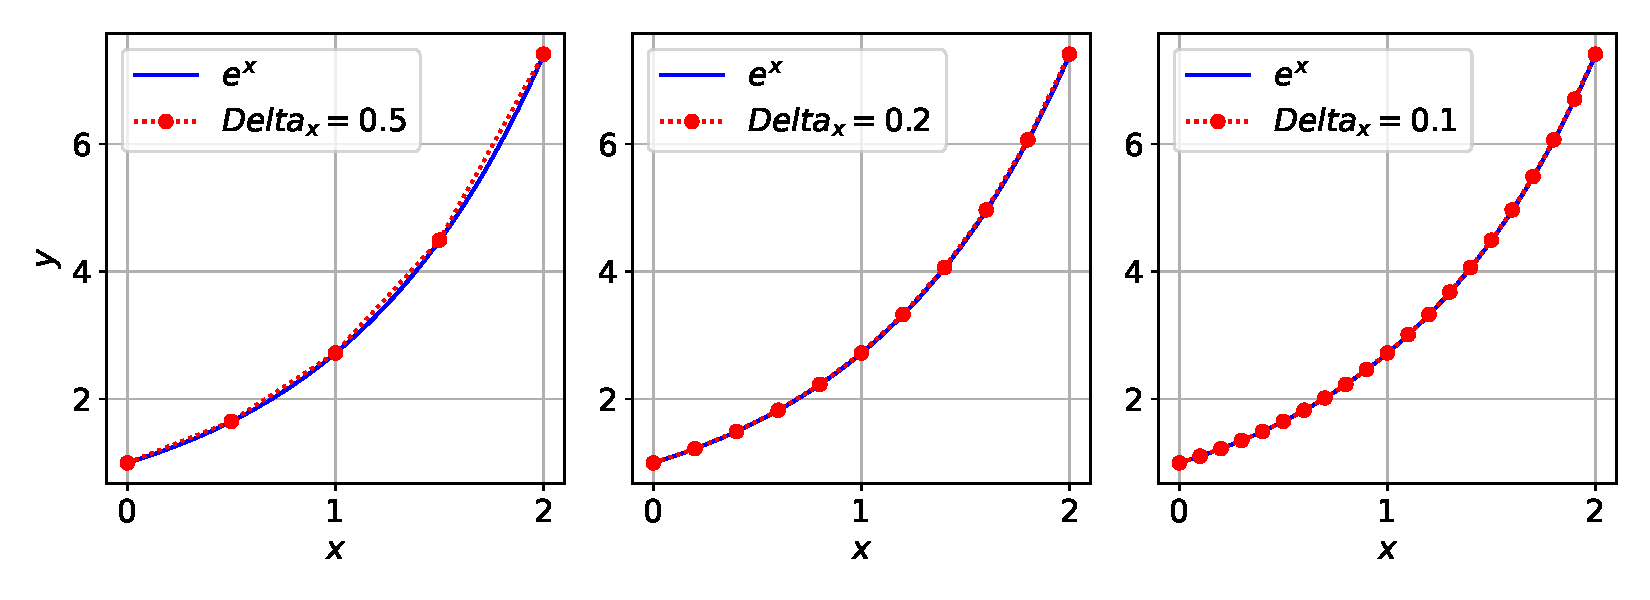
\includegraphics[width=0.8\textwidth]{y=ygraph.pdf}
  \caption{$y' = y$ }
\end{figure}

여기서 sol.sol(x)의 의미는 우리가 지정한 구간에서 구한 sol에서
x의 구간이 촘촘해질수록, 곡률이 더 매끄러워지는 것을 볼 수 있다. 위 sol 함수는 조밀한 출력이라고 하는 다항식 보간을 구현한다. 우리는 원하는 구간내에서의 $y' = y$ 의 상미분 방정식의 해값을 이렇게 구할 수 있다. 이때, 위에서 확인한 Method들은 각기 다른 쓰임이 존재했는데, 고밀도 제어가 필요한 경우의 Method는 오차값이 당연히 작을 것으로 예상되기 때문에 이를 다른 방식을 넣어 오차의 크기를 확인하려고 한다. 먼저 RK45의 경우 오차는 다음과 같다. 

\begin{lstlisting}[language=Python]

def f(x, y):
    return y 

a = solve_ivp(f, [0, 2], [1], method='RK23', dense_output = True)
t = np.linspace(0, 2, 5)

def error(linspace, real_function, a): #a = solve_ivp(f, [0, 2], [1], method='RK45', dense_output = True)
    t = linspace
    i = 0
    y_true = real_function(t)
    b = []
    b.append(*a.sol(t))
    for i, c in enumerate(y_true):
        print((f"error ({t[0]} ~ {t[-1]}) :{y_true[i] - b[0][i]}"))
        
print(error(np.linspace(0, 2, 5), lambda x: np.exp(x), a))
print(error(np.linspace(0, 2, 11), lambda x: np.exp(x), a))
print(error(np.linspace(0, 2, 21), lambda x: np.exp(x), a))
\end{lstlisting}

\begin{lstlisting}[language=Python]
error (0.0 ~ 2.0) :0.0
error (0.0 ~ 2.0) :-4.156935837329456e-06
error (0.0 ~ 2.0) :-2.1237760380099502e-05
error (0.0 ~ 2.0) :-3.1839687372858805e-05
error (0.0 ~ 2.0) :-0.000269366909522617
None
error (0.0 ~ 2.0) :0.0
error (0.0 ~ 2.0) :-3.1015876831963496e-05
error (0.0 ~ 2.0) :-5.8258354160845016e-05
error (0.0 ~ 2.0) :7.074363789305593e-05
error (0.0 ~ 2.0) :0.00013152556591711217
error (0.0 ~ 2.0) :-2.1237760380099502e-05
error (0.0 ~ 2.0) :-0.00017003513837998696
error (0.0 ~ 2.0) :-0.00017410584998689416
error (0.0 ~ 2.0) :0.00011726622438601453
error (0.0 ~ 2.0) :9.377831619072907e-05
error (0.0 ~ 2.0) :-0.000269366909522617
None
error (0.0 ~ 2.0) :0.0
error (0.0 ~ 2.0) :-2.5798541081201165e-10
error (0.0 ~ 2.0) :-3.1015876831963496e-05
error (0.0 ~ 2.0) :-6.603546164218876e-05
error (0.0 ~ 2.0) :-5.8258354160845016e-05
error (0.0 ~ 2.0) :-4.156935837329456e-06
error (0.0 ~ 2.0) :7.074363789305593e-05
error (0.0 ~ 2.0) :0.00012758126396317238
error (0.0 ~ 2.0) :0.00013152556591711217
error (0.0 ~ 2.0) :7.097324756744072e-05
error (0.0 ~ 2.0) :-2.1237760380099502e-05
error (0.0 ~ 2.0) :-6.78728845775467e-05
error (0.0 ~ 2.0) :-0.00017003513837998696
error (0.0 ~ 2.0) :-0.00022855513413411188
error (0.0 ~ 2.0) :-0.00017410584998689416
error (0.0 ~ 2.0) :-3.1839687372858805e-05
error (0.0 ~ 2.0) :0.00011726622438601453
error (0.0 ~ 2.0) :0.00017913007328118624
error (0.0 ~ 2.0) :9.377831619072907e-05
error (0.0 ~ 2.0) :-0.00011247594008079176
error (0.0 ~ 2.0) :-0.000269366909522617
None
\end{lstlisting}

DOP853의 Method의 경우 고밀도 출력에서 많이 사용하는 방식이다. Runge-Kutta Method의 7차 보간 다항식을 구한 것이기 때문에, 높은 정확도를 가지고 있음을 알 수 있다. 실제로 RK45와 비교하였을때 오차크기가 어느정도인지를 확인하면 다음과 같은 결과가 나온다. 
\begin{lstlisting}[language=Python]
error (0.0 ~ 2.0) :0.0
error (0.0 ~ 2.0) :-3.7969912620727797e-06
error (0.0 ~ 2.0) :-9.106313882867312e-05
error (0.0 ~ 2.0) :0.00011141117893398444
error (0.0 ~ 2.0) :3.745382305098133e-05
None
error (0.0 ~ 2.0) :0.0
error (0.0 ~ 2.0) :1.2968071061436603e-11
error (0.0 ~ 2.0) :-6.698338987032315e-06
error (0.0 ~ 2.0) :-8.925274852522591e-07
error (0.0 ~ 2.0) :-2.8524980141941825e-05
error (0.0 ~ 2.0) :-9.106313882867312e-05
error (0.0 ~ 2.0) :-9.637758558689313e-05
error (0.0 ~ 2.0) :2.360861782157997e-05
error (0.0 ~ 2.0) :0.00018518408810930254
error (0.0 ~ 2.0) :0.000180844920722123
error (0.0 ~ 2.0) :3.745382305098133e-05
None
error (0.0 ~ 2.0) :0.0
error (0.0 ~ 2.0) :-6.2232441422338525e-12
error (0.0 ~ 2.0) :1.2968071061436603e-11
error (0.0 ~ 2.0) :-2.7468468677405156e-06
error (0.0 ~ 2.0) :-6.698338987032315e-06
error (0.0 ~ 2.0) :-3.7969912620727797e-06
error (0.0 ~ 2.0) :-8.925274852522591e-07
error (0.0 ~ 2.0) :-7.640067075431745e-06
error (0.0 ~ 2.0) :-2.8524980141941825e-05
error (0.0 ~ 2.0) :-5.993031038409313e-05
error (0.0 ~ 2.0) :-9.106313882867312e-05
error (0.0 ~ 2.0) :-0.00010753605664470811
error (0.0 ~ 2.0) :-9.637758558689313e-05
error (0.0 ~ 2.0) :-5.1220706422050455e-05
error (0.0 ~ 2.0) :2.360861782157997e-05
error (0.0 ~ 2.0) :0.00011141117893398444
error (0.0 ~ 2.0) :0.00018518408810930254
error (0.0 ~ 2.0) :0.0002148185506332112
error (0.0 ~ 2.0) :0.000180844920722123
error (0.0 ~ 2.0) :9.618907302844093e-05
error (0.0 ~ 2.0) :3.745382305098133e-05
None
\end{lstlisting}
예상했던대로, x의 범위중 경계값에 해당하는$x_f$에 가까울수록 오차가 커지는 경우를 위에서 볼 수 있었는데, DOP853의 경우 경계값에서도 $10^{-5}$정도로 비교적 작은 값을 가지는 것을 볼 수 있다. 이외에도 RK23을 사용했을시, 당연하게 45보다 정확도가 떨어지는 것을 볼 수 있다. 







\subsection{Problem Recognition} 
이번에는 $y' = y^2$을 풀어볼 것이다. 이때 $y(0) = -1$라는 값이 주어져 있다. 위 미분방정식의 해는 다음과 같다.
\begin{equation}
y(x) = \frac{-1}{x + 1}
\end{equation}


\subsection{Development of a solution} 
이번에는 LSODA의 방법으로 풀어볼 것이다. 위와 같은 방법으로 코드를 짜면 다음과 같다.

\begin{lstlisting}[language=Python]
def f(x, y):
    return y ** 2

x = np.linspace(0, 5, 16)
sol = solve_ivp(f, [0, 5], [-1], method='LSODA', dense_output = True)

x_true = np.linspace(0, 5, 100)
y_true = -1/(x_true + 1)

plt.figure()
plt.plot(x, *sol.sol(x), ".:r", x_true, y_true, "-b")
plt.legend(["Heun", "$-1/(x + 1)$"])
plt.grid()
plt.xlabel("$x$")
plt.ylabel("$y$")
plt.show()

print(error(x, lambda x: -1/(x + 1), sol))

error (0.0 ~ 5.0) :0.0
error (0.0 ~ 5.0) :0.0005107166633844251
error (0.0 ~ 5.0) :0.0006179231012554132
error (0.0 ~ 5.0) :0.00047276511962957013
error (0.0 ~ 5.0) :0.0004744789574998576
error (0.0 ~ 5.0) :0.00040843393484457646
error (0.0 ~ 5.0) :0.00034521895747735565
error (0.0 ~ 5.0) :0.00035161754804069467
error (0.0 ~ 5.0) :0.0003150987249875281
error (0.0 ~ 5.0) :0.00027771933041087493
error (0.0 ~ 5.0) :0.0002471999955599713
error (0.0 ~ 5.0) :0.00022737869869338123
error (0.0 ~ 5.0) :0.00023806847005869436
error (0.0 ~ 5.0) :0.00021690415046862754
error (0.0 ~ 5.0) :0.000203802342367998
error (0.0 ~ 5.0) :0.00017921160683101456
None
\end{lstlisting}

\subsection{Execution and Assessment}

\begin{figure}[!ht]
  \centering
  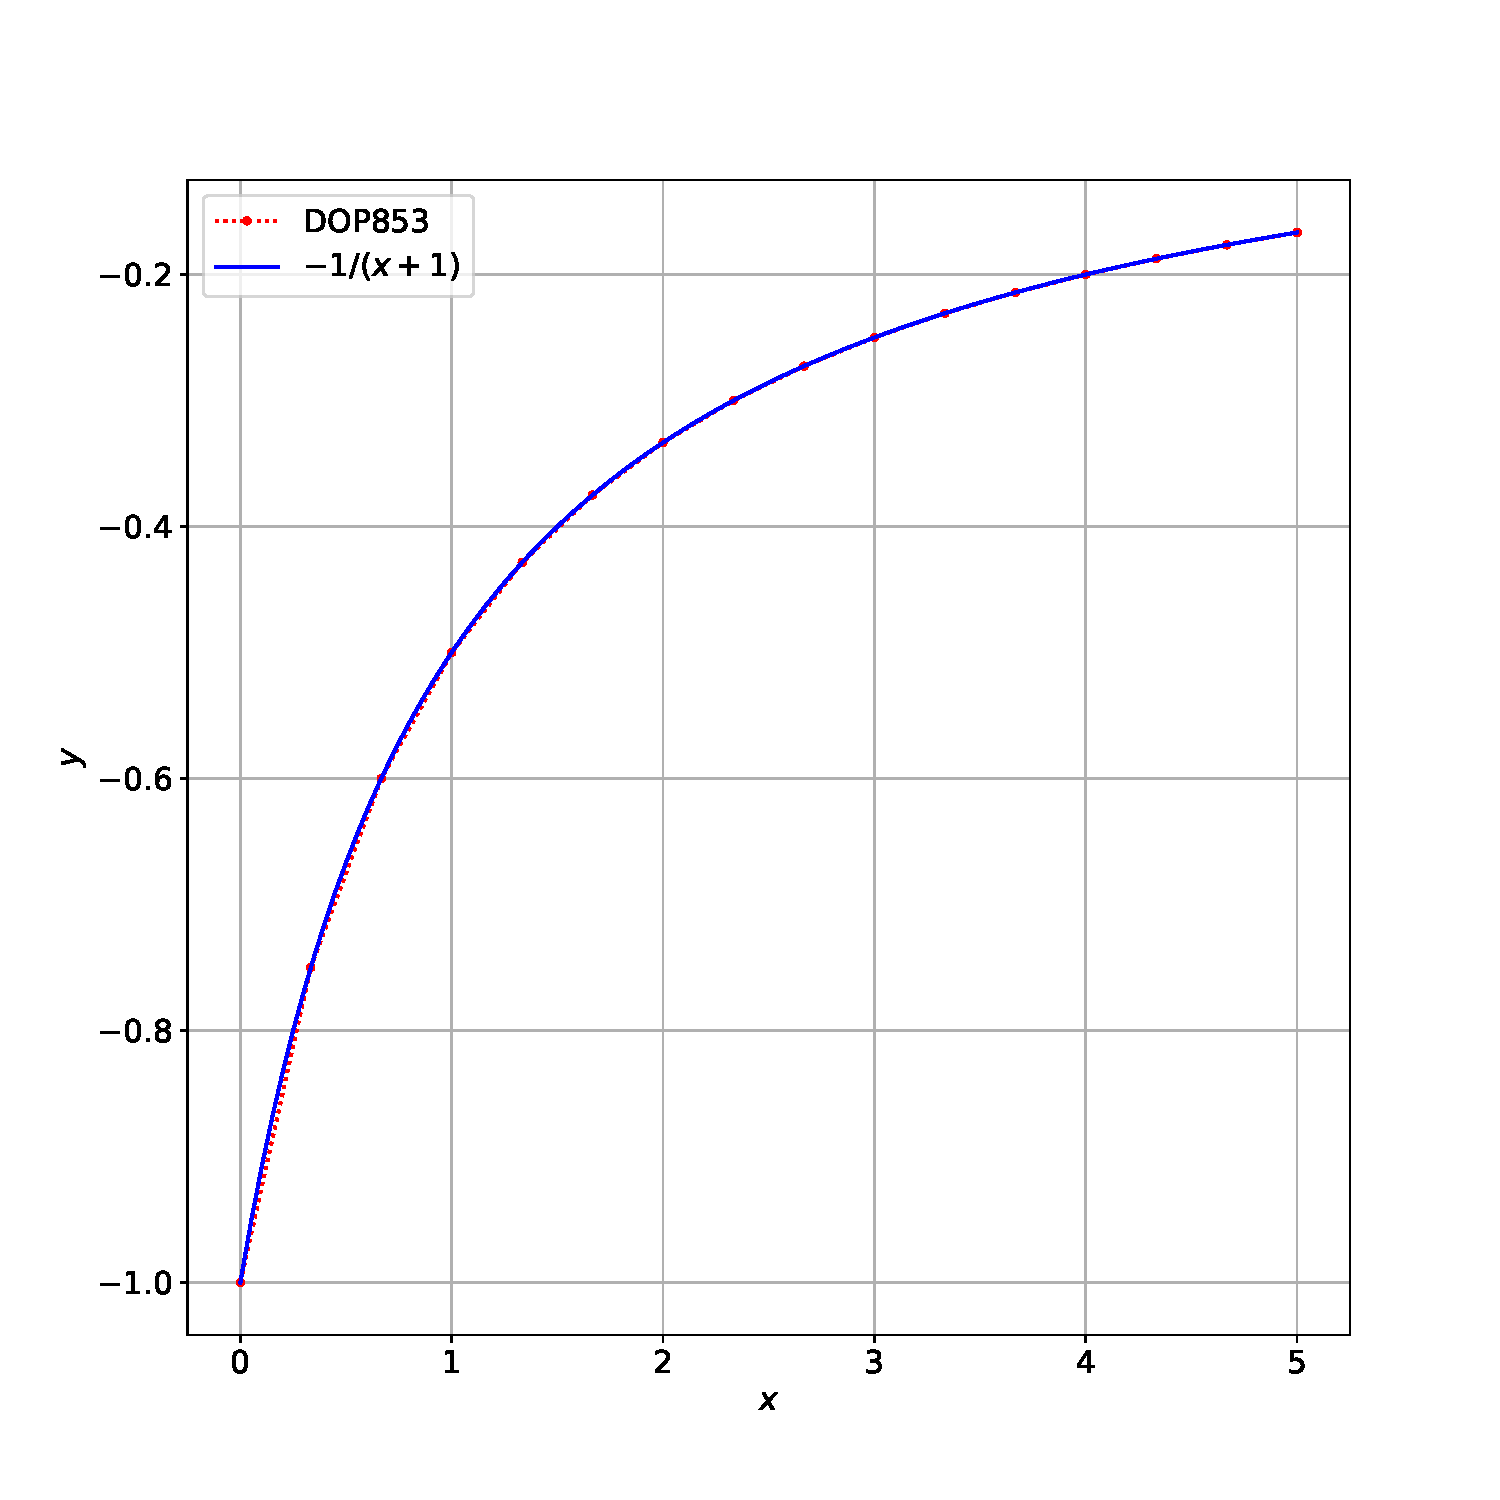
\includegraphics[width=0.5\textwidth]{DOP853.pdf}
  \caption{$y' = y$ }
\end{figure}

예상했던대로, 실제 값과 매우 정교하게 나온 것을 볼 수 있다. 오차를 보면, LSODA의 경우 같은 방식을 RK45로 한 것 보다 오차가 작게 나왔지만 정교한 작업이 필요로 하는 방식에서는 맞지 않는 다는 것을 볼 수 있다. 마찬가지로 DOP853의 방식으로 에러 값을 측정하면 다음과 같이 매우 작은 에러값이 나온다.
\begin{lstlisting}[language=Python]
error (0.0 ~ 5.0) :0.0
error (0.0 ~ 5.0) :4.2580274439707466e-07
error (0.0 ~ 5.0) :1.0940012791893494e-05
error (0.0 ~ 5.0) :-9.795822744851357e-06
error (0.0 ~ 5.0) :-7.599695994731093e-08
error (0.0 ~ 5.0) :9.940520382389906e-07
error (0.0 ~ 5.0) :-1.6535692408115032e-06
error (0.0 ~ 5.0) :7.0241504279699996e-09
error (0.0 ~ 5.0) :4.0402445056209046e-08
error (0.0 ~ 5.0) :9.497284830239927e-07
error (0.0 ~ 5.0) :6.244511590869362e-07
error (0.0 ~ 5.0) :-1.6603436716611242e-06
error (0.0 ~ 5.0) :-1.0250484894225309e-07
error (0.0 ~ 5.0) :-1.560800641509097e-08
error (0.0 ~ 5.0) :-1.385852790858344e-08
error (0.0 ~ 5.0) :-1.2380110631093899e-08
None
\end{lstlisting}










\subsection{Problem Recognition} 
이번에는 뉴턴의 두번째 법칙에 대해서 풀어볼 것이다. 중력상수에 대한 운동방정식은 다음과 같다.
\begin{equation}
\frac{dx^2}{dt^2} = -g
\end{equation}
이 문제의 실제 솔루션은 다음과 같다.
\begin{equation}
x(t) = -\frac{1}{2} gt^2 + v_0 t + x_0
\end{equation}
이때 $x_0 = 0$이며 $v_0 = 1$이 주어졌을 때, 높이와 속도에 대한 그래프를 구해볼 것이다. 범위는 0부터 2/g일때까지 구해야 한다.

\subsection{Development of a solution} 
예제에 나와있는 코드 처럼 2차 미분방정식을 벡터화 한 후, 각각에 대한 값을 구해준다. 이때, Y[1]에 해당하는 값은 v이다. 이 v는 -g로 인해 1차 미분 방정식으로 구해지는 값이기 때문에, 그값이 구해지면, 그것이 다시 Y 변수로 가게 되면서 순차적으로 x도 적분할 수 있게 된다. 또한, 우리는 그래프를 그려야 하는데, sol.sol(t)로 구해지는 값을 리스트 x, v 에 순차적으로 저장하여 그 값을 그래프로 그려볼 것이다. 

\begin{lstlisting}[language=Python]
g = 9.8 # m/s
def F(t, Y): # F = [v, -g], Y = [x, v]
    F = [Y[1], -g]
    return np.array(F)

t    = np.linspace(0, 2/g, 100)
Y_0  = np.array([0, 1])

#Using Zip
x = []
v = []

for a, b in zip(*sol.sol(t)):
    x.append(a)
    v.append(b)
    
sol = solve_ivp(F, [0, 2/g], Y_0, method='LSODA', dense_output = True)



plt.figure(figsize=[11, 4])

plt.subplot(1, 2, 1)
plt.plot(t, -g/2*t**2 + t, '-', t, x, ':k')
plt.legend(["exact", "Heun"])
plt.xlabel("$t$ [s]")
plt.ylabel("$x$ [m]")

plt.subplot(1, 2, 2)
plt.plot(t, -g*t + 1, '-', t, v, ':k')
plt.legend(["exact", "Heun"])
plt.xlabel("$t$ [s]")
plt.ylabel("$v$ [m/s]")

plt.tight_layout()
plt.show()
\end{lstlisting}






\subsection{Execution and Assessment}
\begin{figure}[!ht]
  \centering
  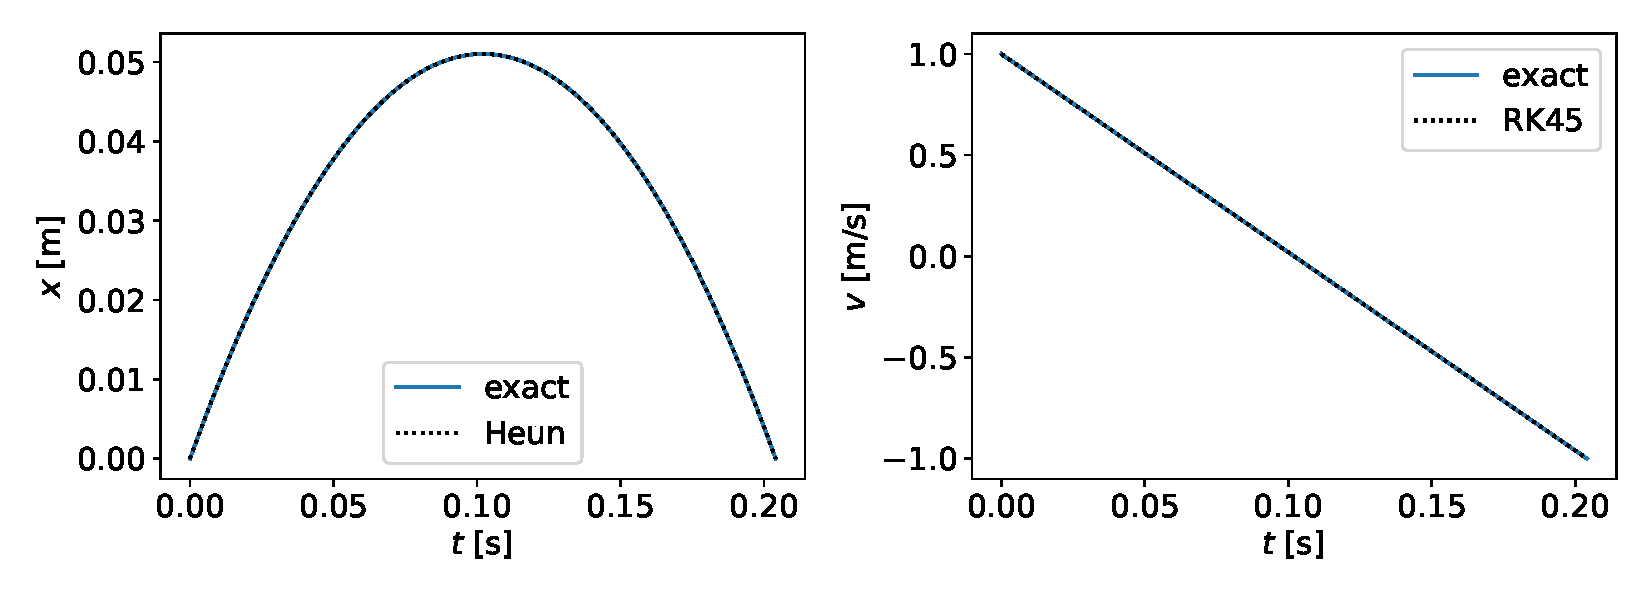
\includegraphics[width=0.7\textwidth]{newton.pdf}
  \caption{Newton's 2nd Law}
\end{figure}

exact 값과 상당히 유사하게 나온 것을 볼 수 있다. 이것에 대한 오차값은 위에서 구한 방식과 동일하게 구하면 되므로 생략한다.

\pagebreak
















\subsection{Shooting Method} 
Shooting method는 초기값 문제로 줄임으로서, 경계값 문제를 해결하는 방법이다. 그것은 경계값 문제의 경계 조건을 만족시키는 해결책을 찾기 전까지 초기값 문제에 대한 해결책을 찾는 것을 포함한다. 우리는 Shooting Method를 이용하여 주어진 시스템의 고유값을 얻을때에 사용할 것이고, 무한한 전위 우물에서 입자의 양자화된 에너지 준위를 얻기 위해서 이것을 적용할 것이다.

\subsection{Problem Recognition} 
Shooting Method를 이용하여 풀어볼 문제는 Particle in a Box이다. 
파동함수 $\psi(x)$위의 전위 우물에 있는 입자는 다음의 2차 미분 방정식으로 설명된다.
\begin{equation}
\frac{d^2\psi}{dx^2} + k^2 \psi = 0
,\qquad 0 < x < L
\end{equation}
여기서 k는 일정하고 이는 입자의 에너지와 관련 있다. 경계값으로 $\psi(0) = \psi(L) = 0$을 가지면 하나의 해를 얻는다. 
\begin{equation}
\psi_n(x) = A \sin k_n x
,\qquad
n = 1, 2, \dots
\end{equation}
여기서 $L = \pi$로 선택하면  $k_n = 1, 2, \dots$이다. 이때 $k_n$은 고유값이다. 이를 Shooting Method를 사용하여 네가지 고유값을 찾아볼 것이다.

이때 고려해야할 사항은 다음과 같다.
\begin{itemize}
\item $x = 0$인 상태에서 미분방정식을 적분시켜야 하고, 초기 조건은 이렇다.
\begin{equation}
\psi_k(0) = 0
    ,\qquad
    \left.\frac{d\psi_k}{dx}\right|_{x = 0} = a
    \end{equation}
    이때, 상수 a는 0이 아닌 임이의 실수이다.
\item 적분 후, 경계조건이 만족하는지 끝 값을 확인한다. 즉, $\psi_k(L) = 0$ 를 만족해야 한다.
\item 만약 만족하지 않으면 k를 다시 체크하고 반복한다.
\end{itemize}

\subsection{Development of a solution} 
먼저, 미분방정식을 풀어주는 해를 구해주고, $\psi_{k}$에 대한 함수를 구하면, $\psi_{k}$에 대한 함수를 다른 함수로 정의하여 그 함수의 x의 근을 찾아준다. 이는 secant 방법을 이용하여 구할 것이다. 이때, secant에서 예상되는 초기값을 [.9, 1.9, 2.9, 3.9]로 지정한 후, 해를 찾아내어, 그것을 x,y에 대한 그림으로 그릴 것이다. 먼저, Scipy로 구해준 해를 리스트에 넣어준 다음, zip과 *함수를 통하여 구하고자 하는 $\psi_{k}$값을 구해줄 것이다. 그 후 이것을 return을 통해 뽑아줄 것이다. 

\begin{lstlisting}[language=Python]
def F(k, x, Y):
    [psi, dpsi] = Y         # Y = [ psi   ,    dpsi/dx  ]
    F = [dpsi, -k**2 * psi] # F = [dpsi/dx, d^2 psi/dx^2]
    return np.array(F)

x, psi = None, None
def wave_function_at_L_away_scipy(k):
    global x, psi
    
    a      = 1
    Y_init = np.array([0, a])
    
    L      = np.pi
    n_divs = 200 
    x      = np.linspace(0, L, n_divs)
    
    #Make Psi list
    psi = []
    sol = solve_ivp(lambda x, Y: F(k, x, Y), [0, L], [0, 1], method='BDF', dense_output = True)
    #psi = [psi for psi, dpsi in sol] 
    #Instead, make a list yourself.
    # The reason for doing this is, in the case of sol.sol(x), the result value is not [1, 2], [3, 4]
    # [1, 3, 5, 6, 7, ...] [1, 3, 5, .... 6, 7] It comes out in two pieces.
    # Since it is not possible to zip too much, it uses a method of storing each element in a single list.
    for c, d in zip(*sol.sol(x)):
        psi.append(c)
    return psi[-1] # we are only interested in psi(L)




# drawing
plt.figure(figsize=[11, 5])

# initial guesses of k to be used in root finder
k_guesses = [.9, 1.9, 2.9, 3.9]
for i, k0 in enumerate(k_guesses): # find first four eigen modes
    n = i + 1

    k = secant_while(wave_function_at_L_away_scipy, [k0, k0 - 0.01],
                     lambda i, xy, dx: abs(dx) >= 1e-7 * abs(xy[0]))

    plt.subplot(2, 2, n)
    plt.plot(x/np.pi, psi, "-r")
    plt.grid()
    if n == 3 or n == 4:
        plt.xlabel("$x/\\pi$")
    if n == 1 or n == 3:
        plt.ylabel("$\\psi$")
    plt.title(f"{n}th eigen mode: $k_{n} = {k:.2f}$")

plt.tight_layout()
plt.show()
\end{lstlisting}

\subsection{Execution and Assessment}
\begin{figure}[!ht]
  \centering
  \includegraphics[width=0.7\textwidth]{particle.pdf}
  \caption{Particle in a box}
\end{figure}
선례에 구했던 하나의 해처럼 sin곡선을 그리면서 진폭과 주기가 달라지는 것을 볼 수 있다.
마찬가지로 이번에는 3차원에서의 그래프도 그려볼 것이다.











\subsection{Problem Recognition} 
이번에 풀어볼 문제는 로렌츠 시스템이다. 특정 매개 변수 값과 초기 조건에 대한 혼란스러운 해결책을 찾는 문제인데, Lolentz Attractor을 상미분 방정식으로 표현하면 다음과 같다.
\begin{equation}
\begin{split}
\begin{aligned}
\frac{dx}{dt} &= 10 (y - x) \\
\frac{dy}{dt} &= x  (28 - z) - y \\
\frac{dz}{dt} &= xy - \frac{8}{3} z \\
\end{aligned}
\end{split}
\end{equation}
이때 초기 조건은 $x(0) = 1$, $y(0) = 0$, $z(0) = 0$ 그리고 $t \in [0, 100]$이다.



\subsection{Development of a solution} 
위에서 풀었던 방식과 동일하게 풀되, 3차원으로 표현하면서 z라는 인수의 값이 하나 더 늘었기 때문에 z까지 총 3개의 공간을 가지는 Y 리스트를 만들어 준다. 또한 Scipy로 푼 x, y 그리고 z의 값을 리스트에 각각 저장하여 이를 plotting하면 된다. 이를 나타내면,

\begin{lstlisting}[language=Python]
def F(t, Y):
    [x, y, z] = Y
    F = [10*(y - x), x*(28 - z) - y, x*y - z*8/3]
    return np.array(F)

Yinit   = np.array([1, 0, 0]) # x0, y0, z0
t       = np.linspace(0, 100, 10001)

x = []
y = []
z = []
sol = solve_ivp(F, [0, 100], Yinit,  method='BDF', dense_output = True)
for a, b, c in zip(*sol.sol(t)):
    x.append(a)
    y.append(b)
    z.append(c)
    

plt.figure(figsize=(6, 6))
ax = plt.subplot(1, 1, 1, projection="3d")
plt.plot(x, y, z, ":b", lw=1)
ax.set_xlabel("$x$")
ax.set_ylabel("$y$")
ax.set_zlabel("$z$")
plt.savefig("lorenz.pdf")
\end{lstlisting}





\subsection{Execution and Assessment}
\begin{figure}[!ht]
  \centering
  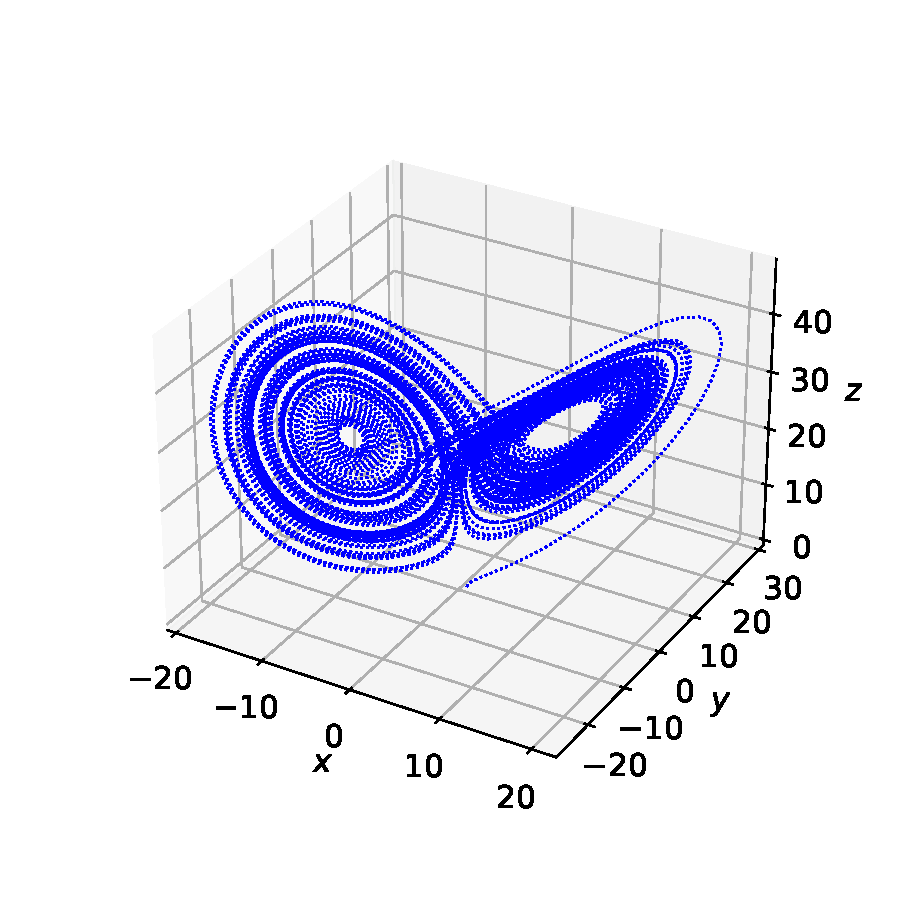
\includegraphics[width=0.7\textwidth]{lorenz.pdf}
  \caption{Lorenz System}
\end{figure}
마찬가지로 우리가 원하는 궤적을 3차원으로 표현하였다. 여기서 주목해야할 것은, 비단 2차원의 식뿐만아니라 3차원의 식도 마찬가지로 미분방정식을 풀 수 있다는 것이고, function을 어떻게 정의하느냐가 핵심인 것을 볼 수 있다.








\subsection{Problem Recognition} 
위와 비슷한 문제로, 우리는 Radioactive Decay 문제를 풀어볼 것이다. 문제는 다음과 같다. Ra이 Rn이 되어 P0가 되는데, $t = 0$이였을때 순수 라듐이였다면, $t = t_{f}$ 일때 Rn의 양을 묻는 문제이다. 이때 $t_f = 10$, $N_{\rm Ra}(0) = 1000$ 그리고 $N_{\rm Rn}(0) = N_{\rm Po}(0) = 0$ 이다.


\subsection{Development of a solution} 
우선 우리는 Function을 먼저 정의해야 한다. 그전에, $N_{Ra}$을 t시간 후 Ra의 원자 갯수라고 하고, 마찬가지로 $N_{Rn}$ 또한 정의한다. 그리고 $\lambda_{\rm Ra},\ \lambda_{\rm Ra} =$ Ra와 Rn의 각기 분해되는 상수라고 하자. 그러면 우리는 $N_{Rn}$ 에 대한 미분방정식을 다음과 같이 정의할 수 있다.
\begin{equation}
\frac{dN_{\rm Ra}}{dt} = -\lambda_{\rm Ra} N_{\rm Ra}
\end{equation}
그리고 이것에 실제 해는 다음과 같다.
\begin{equation}
N_{\rm Ra}(t) = A e^{-\lambda_{\rm Ra} t}
\end{equation}

마찬가지로 Rn의 갯수 변화의 비율은
\begin{equation}
\begin{split}
\begin{aligned}
\frac{dN_{\rm Rn}}{dt} &= -\lambda_{\rm Rn} N_{\rm Rn} + \lambda_{\rm Ra} N_{\rm Ra}
\\
&= -\lambda_{\rm Rn} N_{\rm Rn} + A e^{-\lambda_{\rm Ra} t}
\end{aligned}
\end{split}
\end{equation}
이다. 그리고 이것의 해는

\begin{equation}
\begin{split}
N_{\rm Rn}(t)
=
\left\{
\begin{array}{c}
\displaystyle (A\lambda_{\rm Ra}t + B) e^{-\lambda_{\rm Rn} t}, \lambda_{\rm Ra} = \lambda_{\rm Rn}
\\
\displaystyle A \frac{\lambda_{\rm Ra}}{\lambda_{\rm Rn} - \lambda_{\rm Ra}} e^{-\lambda_{\rm Ra}t} + B e^{-\lambda_{\rm Rn} t} , \lambda_{\rm Ra} \ne \lambda_{\rm Rn}
\end{array}
\right.
\end{split}
\end{equation}
이다. 마지막으로 P0의 변화 비율은 다음과 같이 구할 수 있다.
\begin{equation}
\frac{dN_{\rm Po}}{dt} = \lambda_{\rm Rn} N_{\rm Rn}
\end{equation}
위에서 구한 방식대로, f를 3가지 요소에 대해 정의하고, 주어진 상수를 대입하여 함수를 정의하고, 앞서 정의한 실제 해의 값도 정의해준다.  P0의 실제 값의 경우, 질량보존법칙을 이용하여 따로 구하지 않고 전체 값에다가 Ra과 Rn을 빼줌으로써 구해준다. 
\begin{lstlisting}[language=Python]
# constants
lam_Ra, lam_Rn         = 1, 1       # change this accordingly
N_Ra_0, N_Rn_0, N_Po_0 = 1000, 0, 0

# dY/dt
def F(t, Y): # F = [dN_Ra/dt, dN_Rn/dt, dN_Po/dt], Y = [N_Ra, N_Rn, N_Po]
    N_Ra, N_Rn, N_Po = Y
    dN_Ra = -lam_Ra * N_Ra
    dN_Rn = -lam_Rn * N_Rn + lam_Ra * N_Ra
    dN_Po = +lam_Rn * N_Rn
    return np.array([dN_Ra, dN_Rn, dN_Po])

# solve ODE
t   = np.linspace(0, 10, 1000)
Y_0 = np.array([N_Ra_0, N_Rn_0, N_Po_0])


N_Ra = []
N_Rn = []
N_Po = []
sol = solve_ivp(F, [0, 10], Y_0,  method='RK45', dense_output = True)
for a, b, c in zip(*sol.sol(t)):
    N_Ra.append(a)
    N_Rn.append(b)
    N_Po.append(c)


# exact solution
N_Ra_true = N_Ra_0*np.exp(-lam_Ra*t)

if lam_Ra == lam_Rn:
    N_Rn_true = (N_Ra_0*lam_Ra*t + N_Rn_0)*np.exp(-lam_Rn*t)
else:
    N_Rn_true = N_Ra_0*lam_Ra/(lam_Rn - lam_Ra) * (np.exp(-lam_Ra*t) - np.exp(-lam_Rn*t))

# total number of atoms at any given time must be invariant
N_Po_true = N_Ra_0 - (N_Ra_true + N_Rn_true)



    
# draw
plt.figure(figsize=[8, 4])
#
plt.plot(t, N_Ra, label="Radium")
plt.plot(t, N_Ra_true, "--k", lw=1)
#
plt.plot(t, N_Rn, label="Radon")
plt.plot(t, N_Rn_true, "--k", lw=1)
#
plt.plot(t, N_Po, label="Polonium")
plt.plot(t, N_Po_true, "--k", lw=1)
#
plt.xlabel("$t$")
plt.ylabel("Count")
plt.legend()
plt.grid()
plt.savefig('Radium.pdf')
\end{lstlisting}






\subsection{Execution and Assessment}
\begin{figure}[!ht]
  \centering
  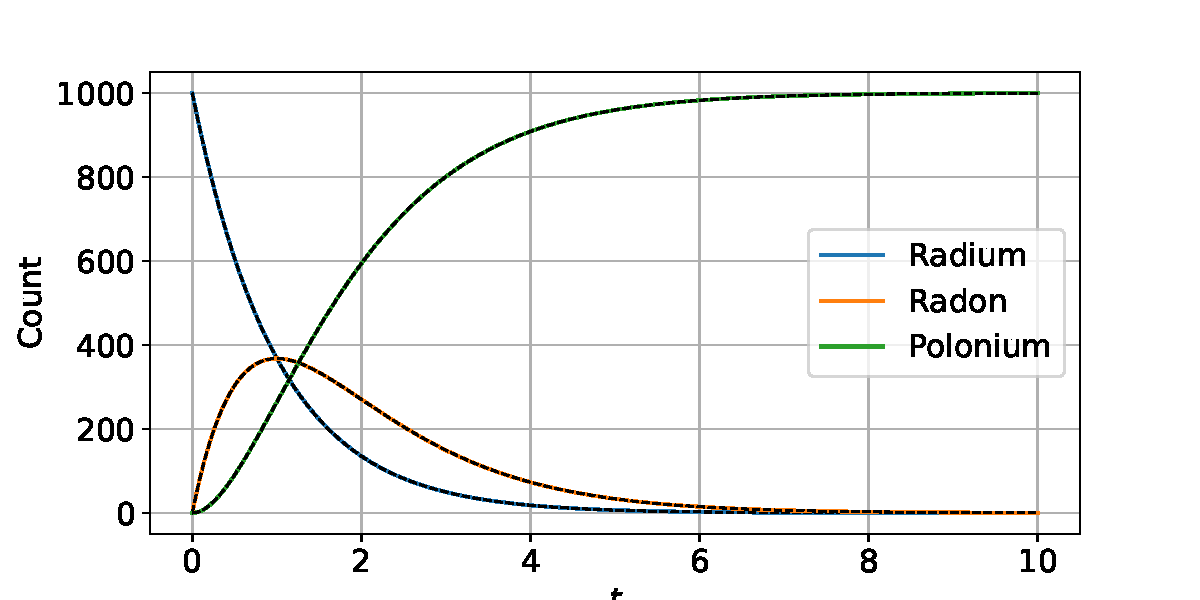
\includegraphics[width=0.7\textwidth]{Radium.pdf}
  \caption{Radioactive Decay}
\end{figure}
우리가 원하는 결과값이 나왔다. 검은 색 줄에 해당하는 실제값과 우리가 구한 Ra, Rn 그리고 P0의 원자 갯수의 양이 잘 맞아 떨어지는 것을 볼 수 있다.










\section{Three-body Problem}
\subsection{Problem Recognition} 
지구-달 시스템을 공전하는 아폴로 우주선처럼, 작은 질량의 물체가 훨씬 더 큰 질량을 가진 두개의 다른 물체를 공전하는 Three-body를 풀어볼 것이다. 좌표계는 지구-달 축을 따라 고정되어 있어, 세 물체가 평면에서 2차원 데카르트 좌표계에 있다. 원점은 두개의 무거운 물체의 질량 중심에 있으며 모든 거리 측정은 지구와 달 사이의 거리가 1이 되도록 정규화된다. 따라서 만약 $\mu$는 달의 질량과 지구의 질량의 비율이므로 달과 지구는 각각 다음의 좌표에 위치한다. (1 - $\mu$, 0) , (-$\mu$, 0). 그리고 좌표계는 달이 지구를 중심으로 회전함에 따라 회전한다. 이 상황은 아래의 다이어 그램에 설명된다.
\begin{figure}[!ht]
  \centering
  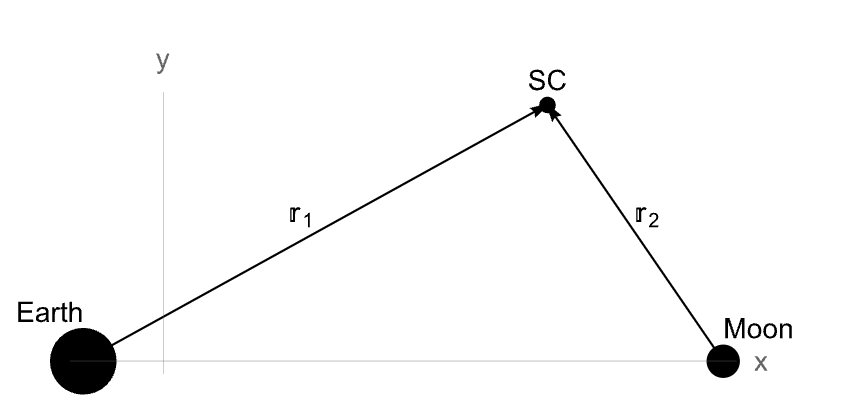
\includegraphics[width=0.7\textwidth]{Three.png}
  \caption{Three-Body Diagram}
\end{figure}
또한 세 번째 물체인 아폴로 우주선은 다른 두 물체에 비해 무시할 수 있는 질량을 가진다. 그리고 이는 t에 대한 함수로 $(x(t), y(t))$로 나타낼 수 있으며, 이 우주선의 위치에 대한 미분 방정식은 뉴턴의 운동 법칙과 중력의 역제곱 법칙에서 파생되어 다음과 같다.
\begin{equation}
\begin{split}
\begin{aligned}
x'' &= 2y' + x - \frac{\mu^* (x + \mu)}{r_1^3} - \frac{\mu (x - \mu^*)}{r_2^3} \\
y'' &= -2x' + y - \frac{\mu^* y}{r_1^3} - \frac{\mu y}{r_2^3} \\
\end{aligned}
\end{split}
\end{equation}
여기서 
\begin{equation}
\begin{split}
\begin{aligned}
\mu &= \frac{1}{81.45} \\
\mu^* &= 1 - \mu \\
r_1^2 &= (x + \mu)^2 + y^2 \\
r_2^2 &= (x - \mu^*)^2 + y^2
\end{aligned}
\end{split}
\end{equation}
이때 경우 1,2에 대한 초기 조건은 다음과 같다.
\begin{equation}
\begin{split}
\begin{aligned}
(\mathrm{I}) \quad &\left\{
\begin{array}{l}
x(0) = 1.2, & y(0) = 0, \\
x'(0) = 0, & y'(0) = -1.04935751, \\
\end{array}
\right.
\\\\
(\mathrm{II}) \quad &\left\{
\begin{array}{l}
x(0) = 0.994, & y(0) = 0, \\
x'(0) = 0, & y'(0) = -2.03173262956, \\
\end{array}
\right.
\end{aligned}
\end{split}
\end{equation}
해결해야되는 순차적 목표는 다음과 같다.
\begin{itemize}
\item 이 문제를 ODE의 1차 시스템으로 변환한다.
\item 적응형 단계 크기 제어와 함께 4차 Runge-Kutta 방법을 사용하여 문제를 해결하고 다양한 허용오차를 실험한다. 결과를 x-y 초기 조건의 두 세트에 대하여 각각 plotting 한다.
\item 한 세트의 초기 조건에 대해 적분이 진행됨에 따라 ODE루틴에서 사용하는 Stepsize를 확인하고 Stepsize는 언제 작아지거나 커지는지 확인하여라.
\item이 ODE 시스템에는 많은 흥미로운 솔루션이 있다. 초지 조건의 다양한 값으로 실험하고 다양한 궤도 동작에 대해 확인해보자.
\end{itemize}
이 문제에서 먼저 풀어야될 절차는,  먼저 주어진 $(x(t), y(t))$에 대한 2차 상미분 방정식을 1차 시스템으로 변환시키고, 이를 적응형 단계 크기 제어 방법과 Runge-Kutta 방법을 통해 적분하여 $(x(t), y(t))$의 값을 구한다. 그리고 이것을 초기조건과 맞추어 그래프로 그린 후 허용오차에 따른 그래프 변이나 초기조건에 따른 다양한 실험 변화에 대해서 분석해야 한다.

\subsection{Development of a solution} 
문제를 풀기 전, 가장 고려해야 할 것은 예제에서도 봤듯이, Function을 어떻게 정하는가가 중요하다. 우리는 위 식,
\begin{equation}
\begin{split}
\begin{aligned}
x'' &= 2y' + x - \frac{\mu^* (x + \mu)}{r_1^3} - \frac{\mu (x - \mu^*)}{r_2^3} \\
y'' &= -2x' + y - \frac{\mu^* y}{r_1^3} - \frac{\mu y}{r_2^3} \\
\end{aligned}
\end{split}
\end{equation}
에서 2차 상미분 방정식을 1차로 바꿔야 하는데 그럴려면, 먼저 F를 이렇게 생각해 볼 수 있다.
\begin{equation}
\mathbf
\quad\mathrm
\mathbf{F}(t, \mathbf{Y}) =
\begin{pmatrix}
\frac{dx}{dt}  \\
\frac{dy}{dt} \\
\frac{dv_{x}}{dt} \\
\frac{dv_{y}}{dt} \\
\end{pmatrix}
\end{equation}
문제를 풀기 전, 변수값과 상수값을 파악하며 def 함수로 계속해서 변하는 변수와 그 밖에 상수로 지정할 변수를 구분해야 한다. 즉, F(t, Y)에서 Y에 들어갈 변수$x, y, v_{x}, v_{y}$가 정의되고 이것으로  $F_{x}$와 $F_{y}$를 정의하여 return을 시켜야 하는 Function을 만들어야 한다. 그럴려면 $r_{1}$값과 $r_{2}$ 값을 정의를 해야하는데, 이는 x와 y에 따라 변하는 변수이므로, 함수 내에서 계산해야 하는 변수이다. 따라서 함수 안에는  $r_{1}$값과 $r_{2}$ 값이 정의 되어야 하고, $F_{x}$와 $F_{y}$에 대한 계산 값도 정의되어야 한다. 하지만, $\mu$의 경우 이미 정해져 있는 상수이기 때문에 우리가 미분 방정식을 풀 때 사용하는 모듈에서 필요한 초기 조건들과 tlim, abstol, reltol 값들을 같이 지정해주면 된다. 즉, 코드로 나타내면 다음과 같다.

\begin{lstlisting}[language=Python]
h_list = hs #hs 
ylist_list = ylist # ylist 
#ylist_list[2:] - ylist_list[1:] Since the beginning is big, increase the same value.
ylist_2 = ylist_list[2:] # List starting with 2
ylist_2 = np.append(ylist_2, ylist_list[-1]) # Add Last Element
diff_ylist_err = []
a = 0
b = 70

for i, j in zip(ylist_2, ylist_list[1:]):
    diff_ylist_err.append(abs(i - j))

h_list_2 = h_list[2:]
h_list_2.append(h_list[-1])
diff_h_list = []

for i, j in zip(h_list_2, h_list):
    diff_h_list.append(i - j)
    
#rel_err_list[2:] - rel_err_list[1:] 
rel_err_2 = rel_err_list[2:] 
rel_err_2.append(rel_err_list[-1]) 
diff_rel_err = []

for i, j in zip(rel_err_2, rel_err_list[1:]):
    diff_rel_err.append(i - j)

    
#Plotting (x, y)!!
plt.figure(figsize=[10, 10])
plt.semilogy(xlist[a:b], diff_ylist_err[a:b], ".:r",xlist[a:b], rel_err_list[a:b], ".:b")


plt.grid()
plt.xlabel("$x$")
plt.ylabel("$\delta$")
#plt.title("h & rel_{err} Graph")
plt.legend(["$\delta_{1}$ - $\delta_{0}$", "h"], fontsize=12)
plt.tight_layout()
plt.show()
\end{lstlisting}
먼저 적응형 스텝제어를 이용하여 4차 Runge-Kutta 방식을 이용했는데, 
충분한 궤도를 보기 위해 tlim은 $[0, 5 * \pi]$로 선정하고, error 값을 낮추기 위해 abstol과 reltol 모두 $10^-9$으로 정의했다. 또한, 인공위성의 질량은 1이라고 가정하였다. 그렇게 해서 코드를 실행하면 다음과 같이 나온다.


\subsection{Execution and Assessment}
\begin{figure}[!ht]
  \centering
  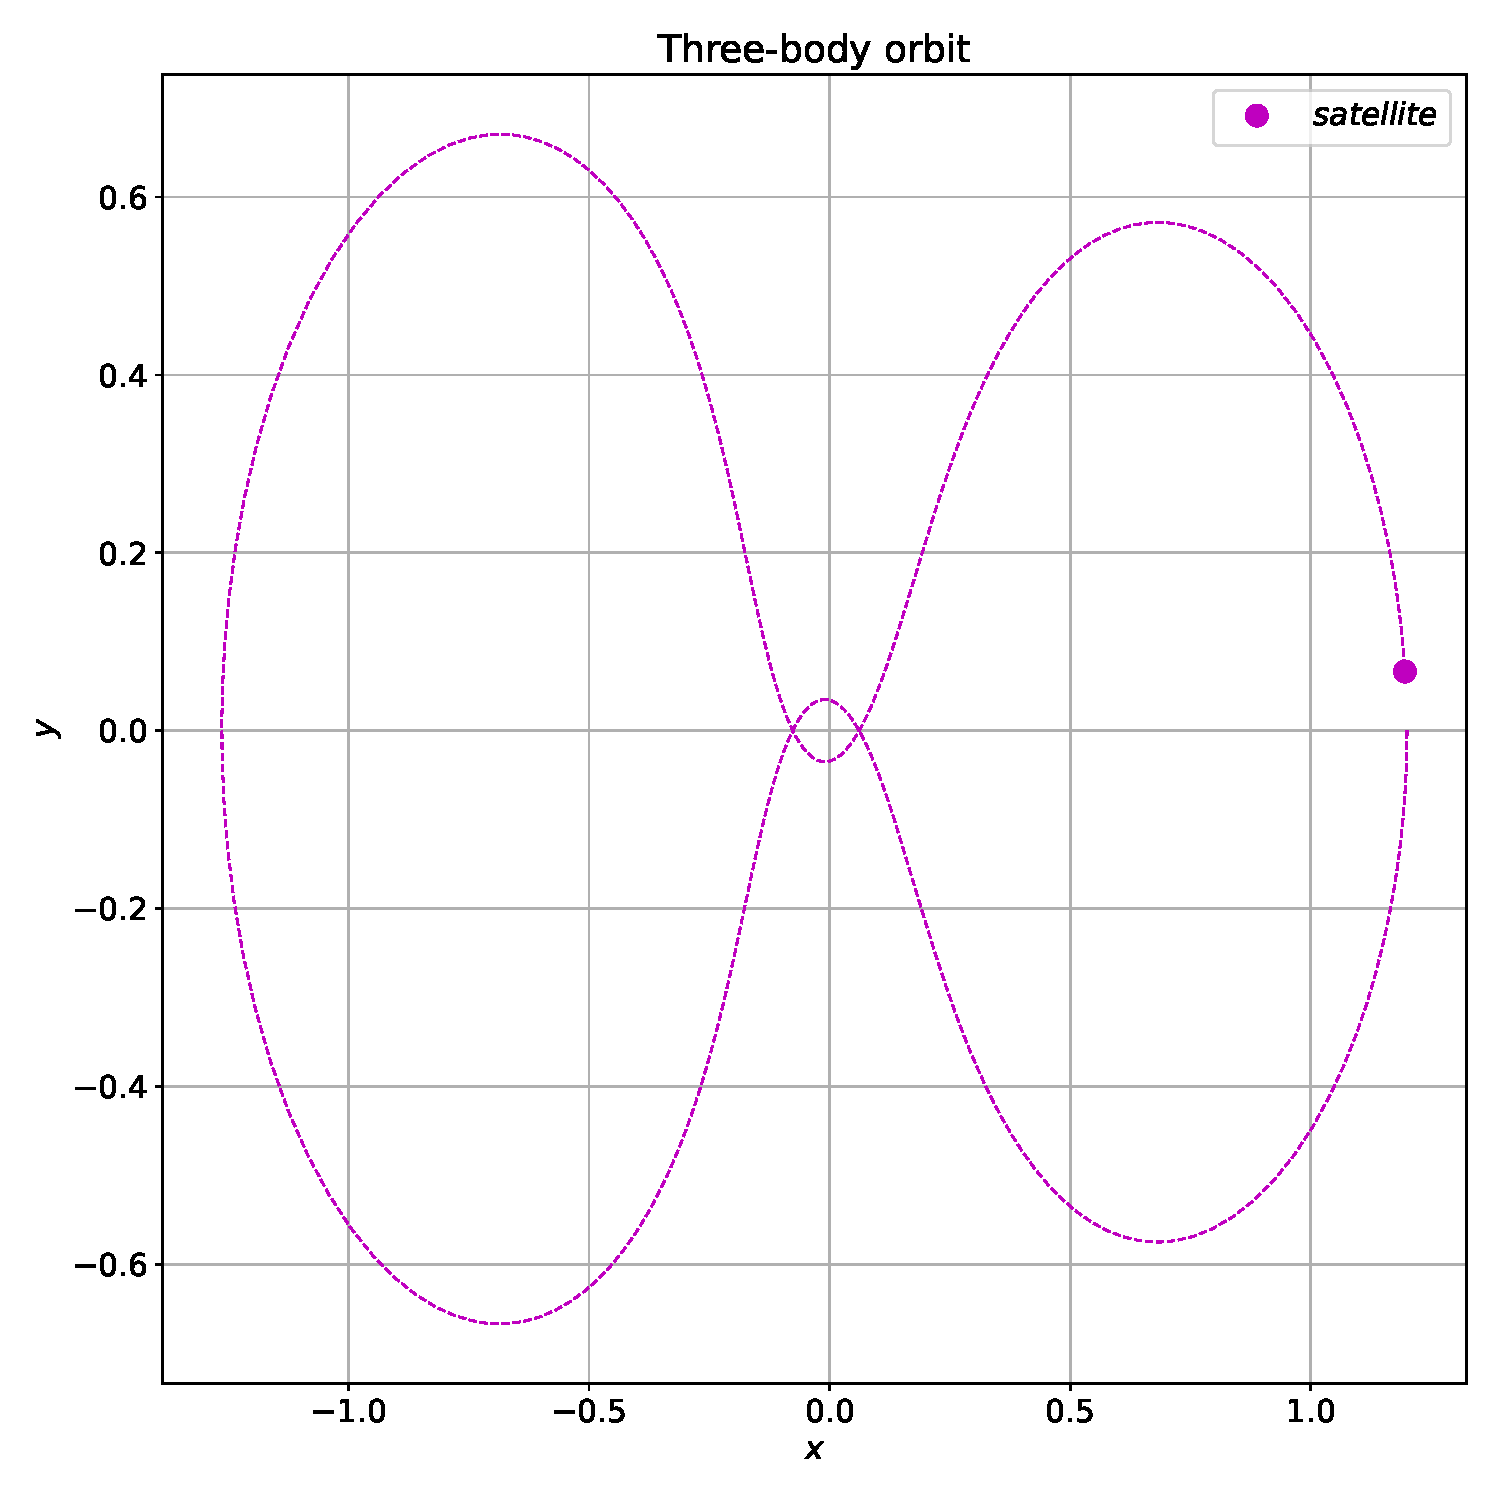
\includegraphics[width=0.5\textwidth]{Three1.pdf}
  \caption{1st Initial Value}
\end{figure}
앞서 첫번째 케이스를 초기값으로 잡으면 Figure 8 과 같은 궤도가 그려진다. 만약 여기서 초기값을 두번째 케이스로 바꾸게 되면 Figure9처럼 된다.
\begin{figure}[!ht]
  \centering
  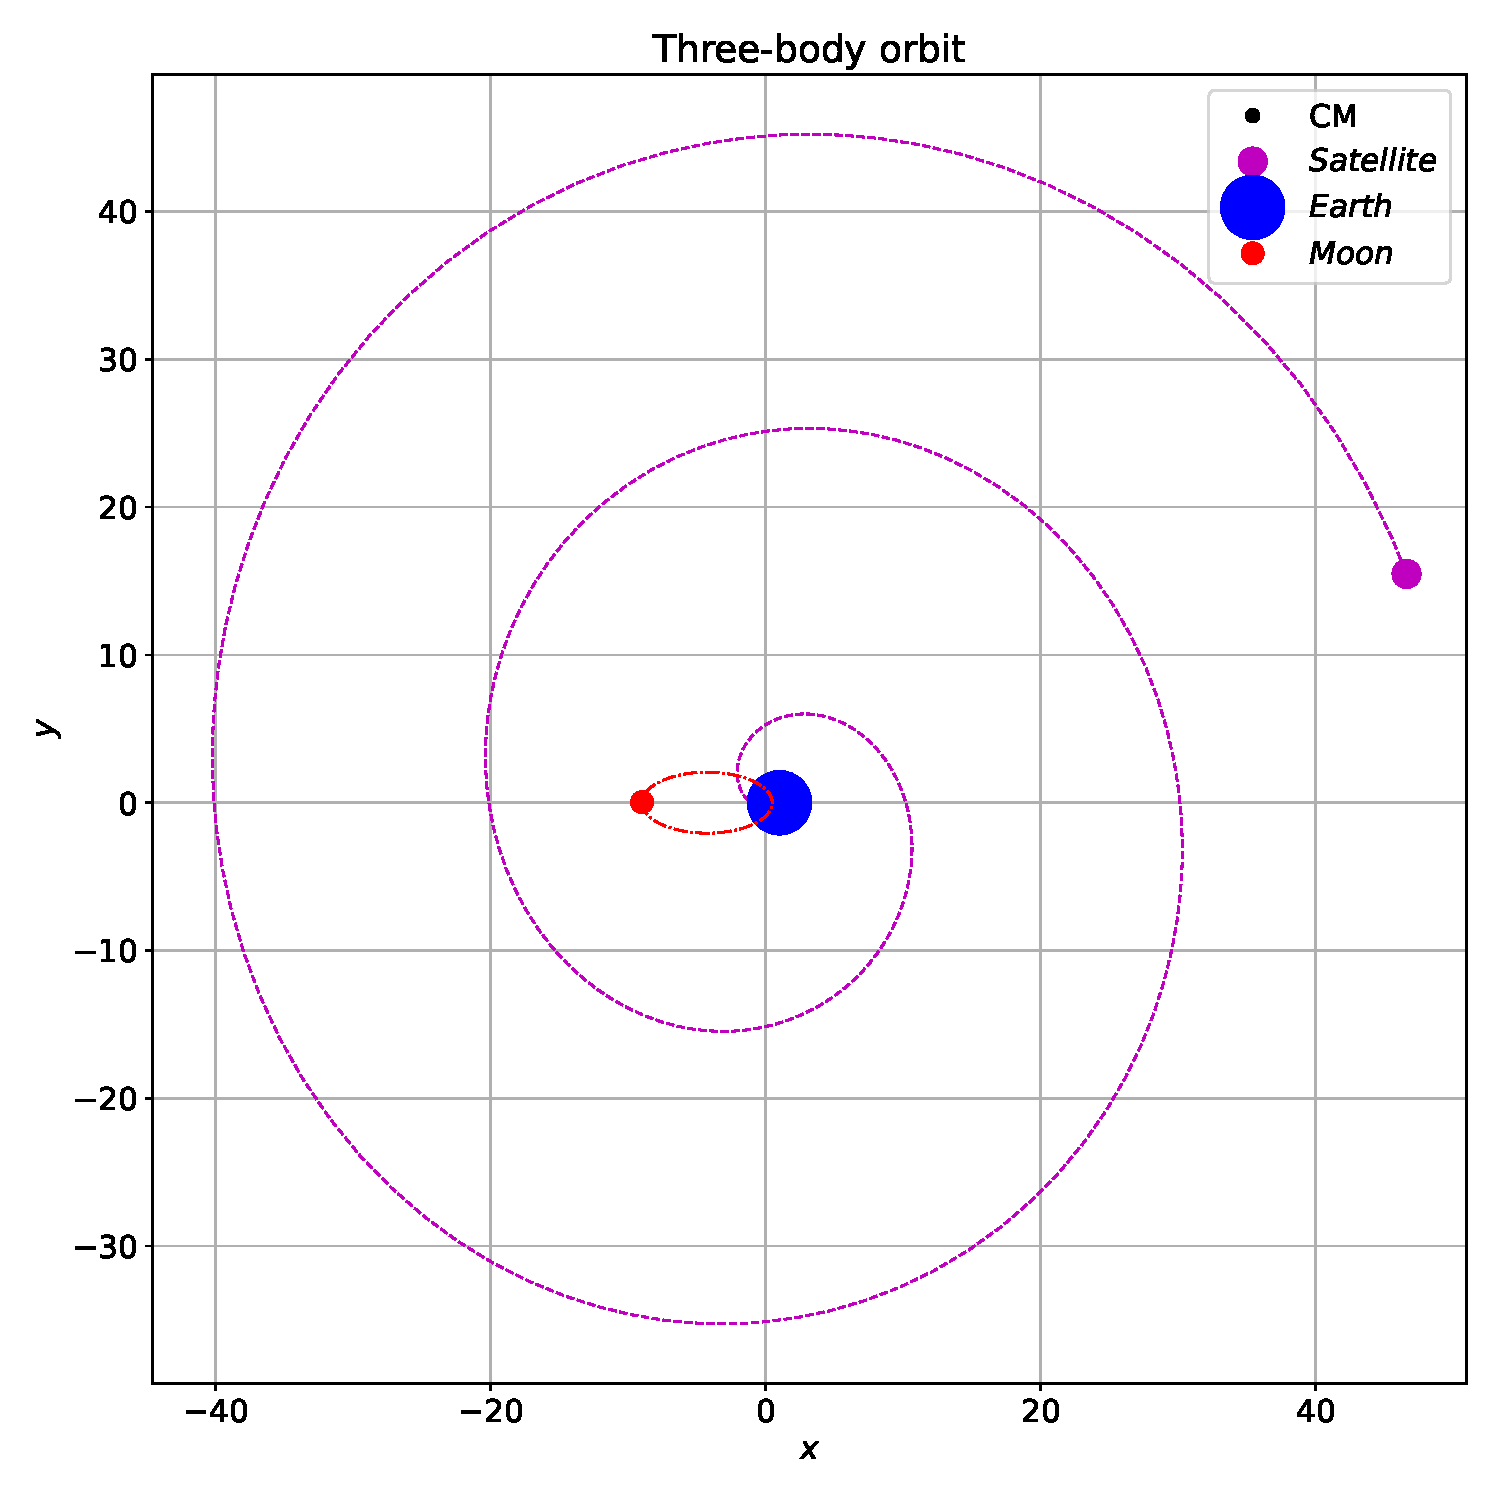
\includegraphics[width=0.5\textwidth]{Three2.pdf}
  \caption{2nd Initial Value}
\end{figure}
여기서 볼 수 있듯이, 초기값에 따라서 궤도의 모양과 크기 등이 전부 변할 수 있다. 이점을 참고하여 만약 오차가 변하면 그래프가 어떻게 변할지도 확인해보자.
먼저 여기서는 abstol = reltol = $10^-3$으로 두었을 때이다. 그러면 그래프는 Figure10이 된다. 만약 이것보다 약간 더 작아지면 즉, abstol = reltol = $10^-5$ 인 경우 Figure 11이 된다.

\begin{figure}[!ht]
  \centering
  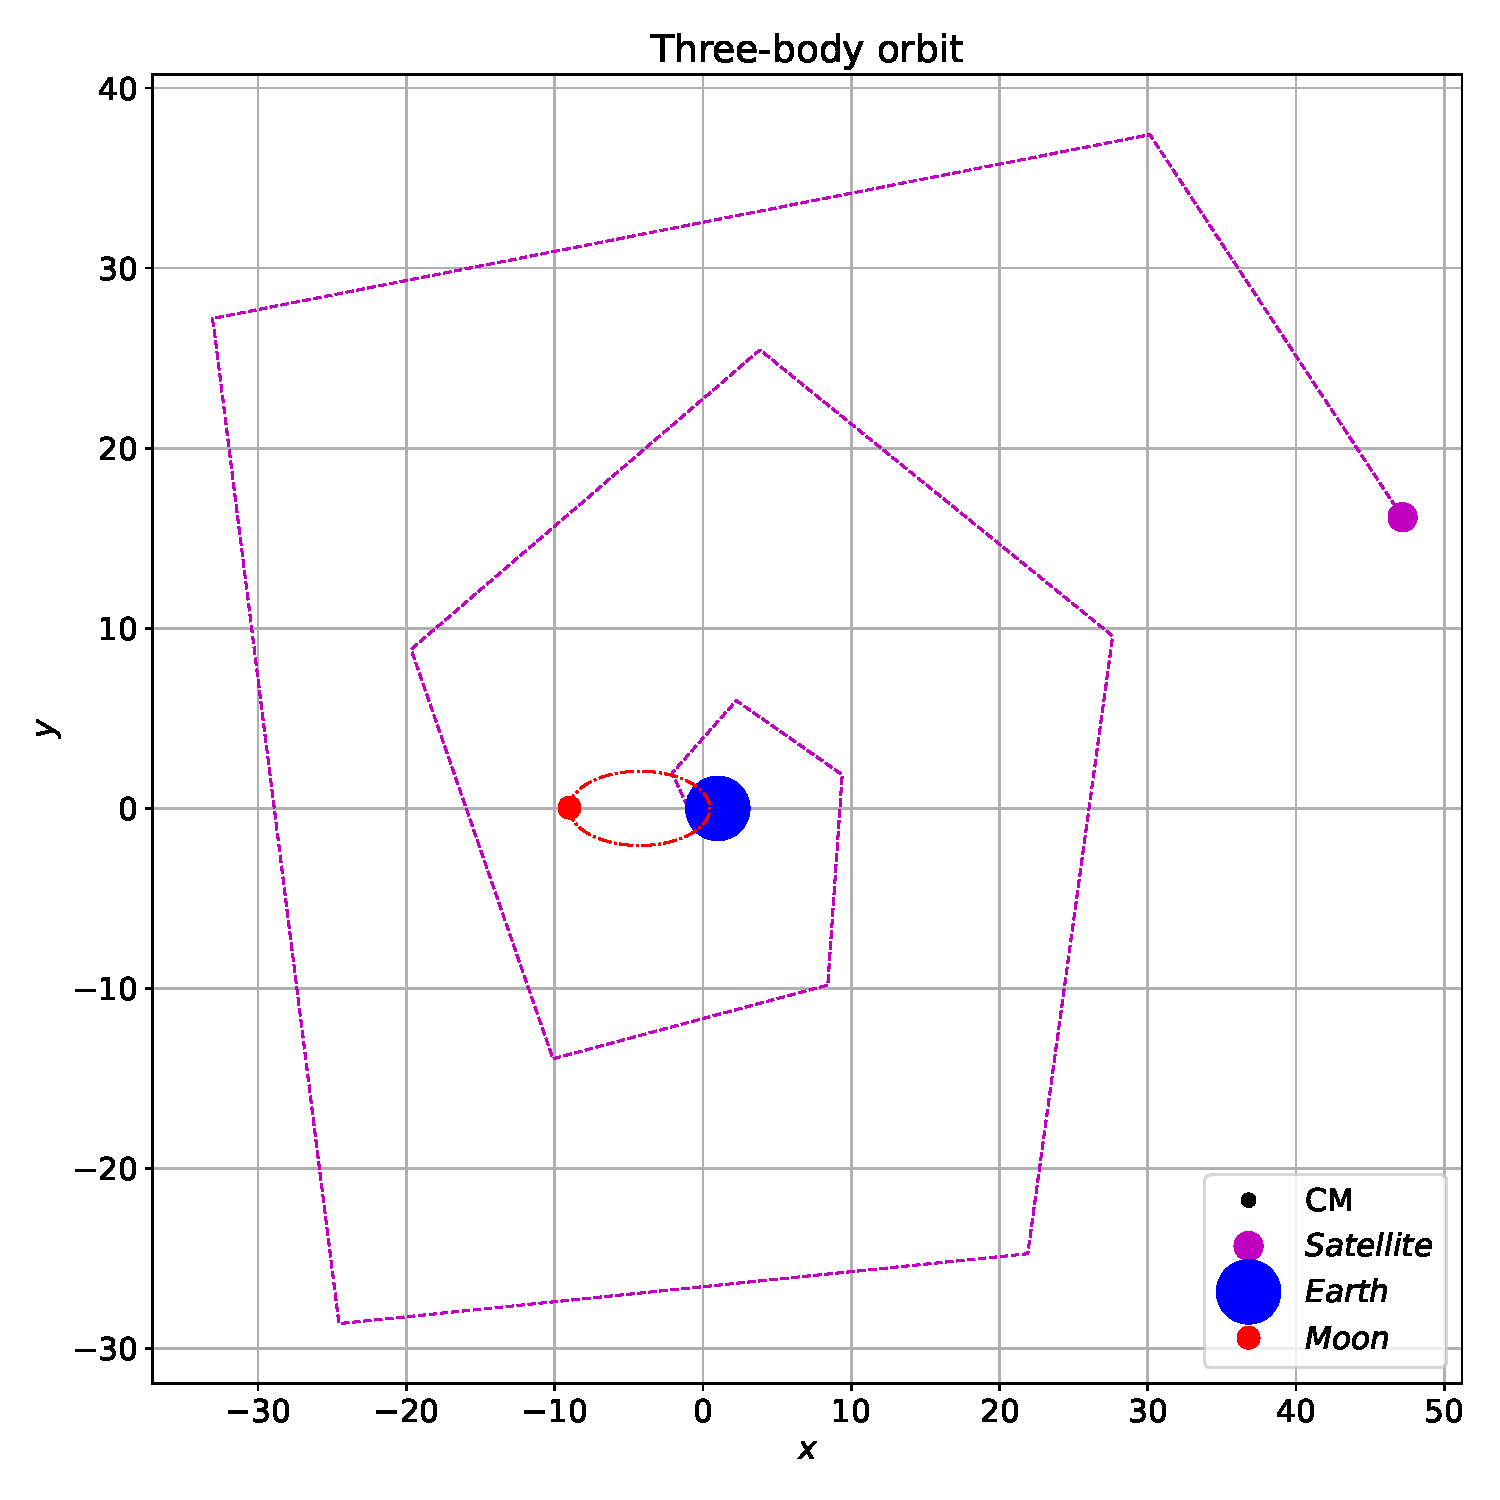
\includegraphics[width=0.5\textwidth]{Three3.pdf}
  \caption{Abstol = Reltol = $10^-3$}
\end{figure}

\begin{figure}[!ht]
  \centering
  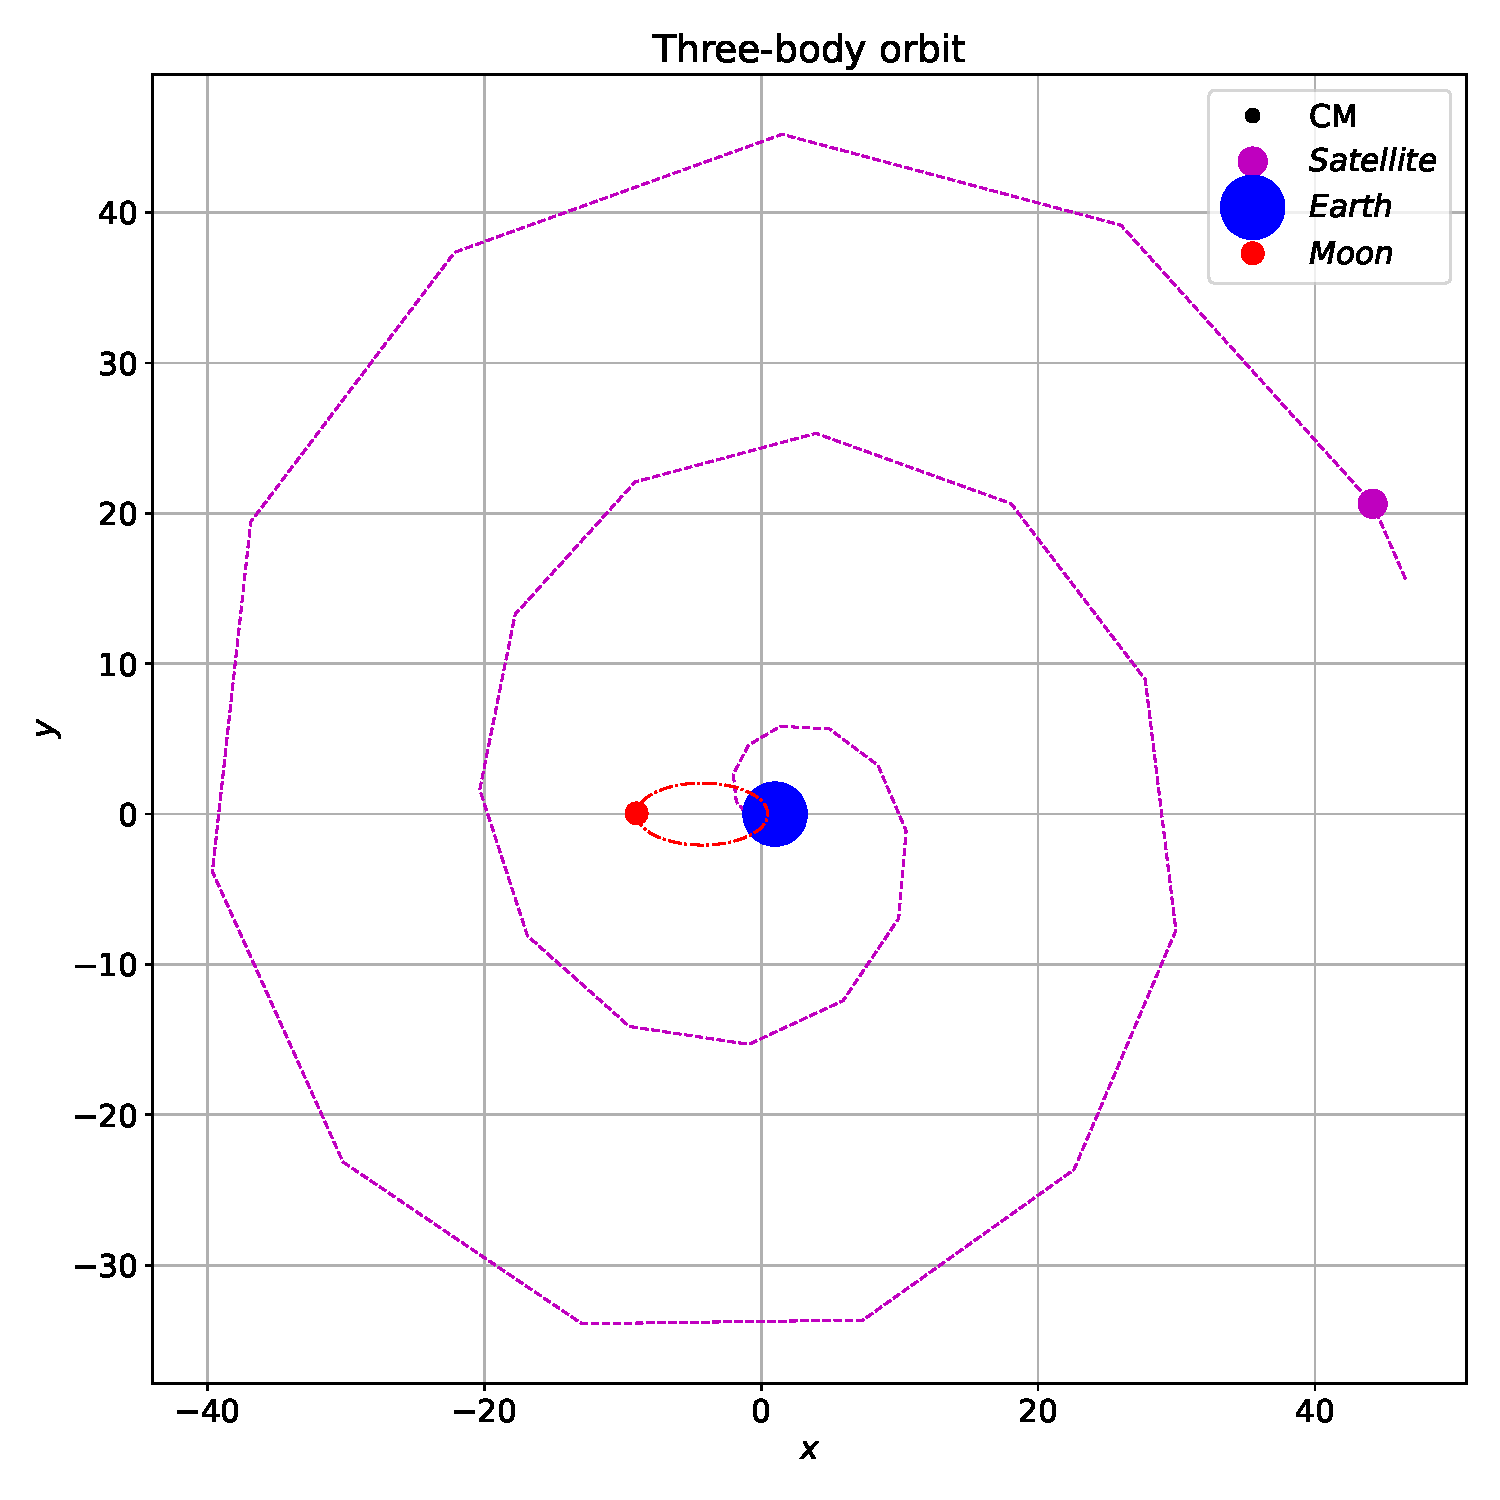
\includegraphics[width=0.5\textwidth]{Three4.pdf}
  \caption{Abstol = Reltol = $10^-5$}
\end{figure}
외에도 abstol 과 reltol 값을 다르게 하면, 둘중 어느 한값이 매우 작다 하더라도, 그래프가 매끄럽지 않게 된다. 즉, 두개 다 작은 값을 가질때 두개의 값의 차이가 적을 수록 그래프는 더 매끄럽고 곡선을 그리게 된다.  이때 한 세트의 초기 조건에 대해 적분이 진행됨에 따라 ODE루틴에서 사용하는 Stepsize를 확인하고 Stepsize는 언제 작아지거나 커지는지 확인해보자. 우선 위성의 위치와 Stepsize h에 대한 관계는 다음 그래프로 그려진다.
\begin{lstlisting}[language=Python]
plt.figure(figsize=[10, 10])
plt.semilogy(xlist, ylist, ".:r",xlist, hs, ".:b")
plt.legend(["location of settlelite", "h"], fontsize=12)

plt.savefig("xandhs.pdf")
\end{lstlisting}

\begin{figure}[!ht]
  \centering
  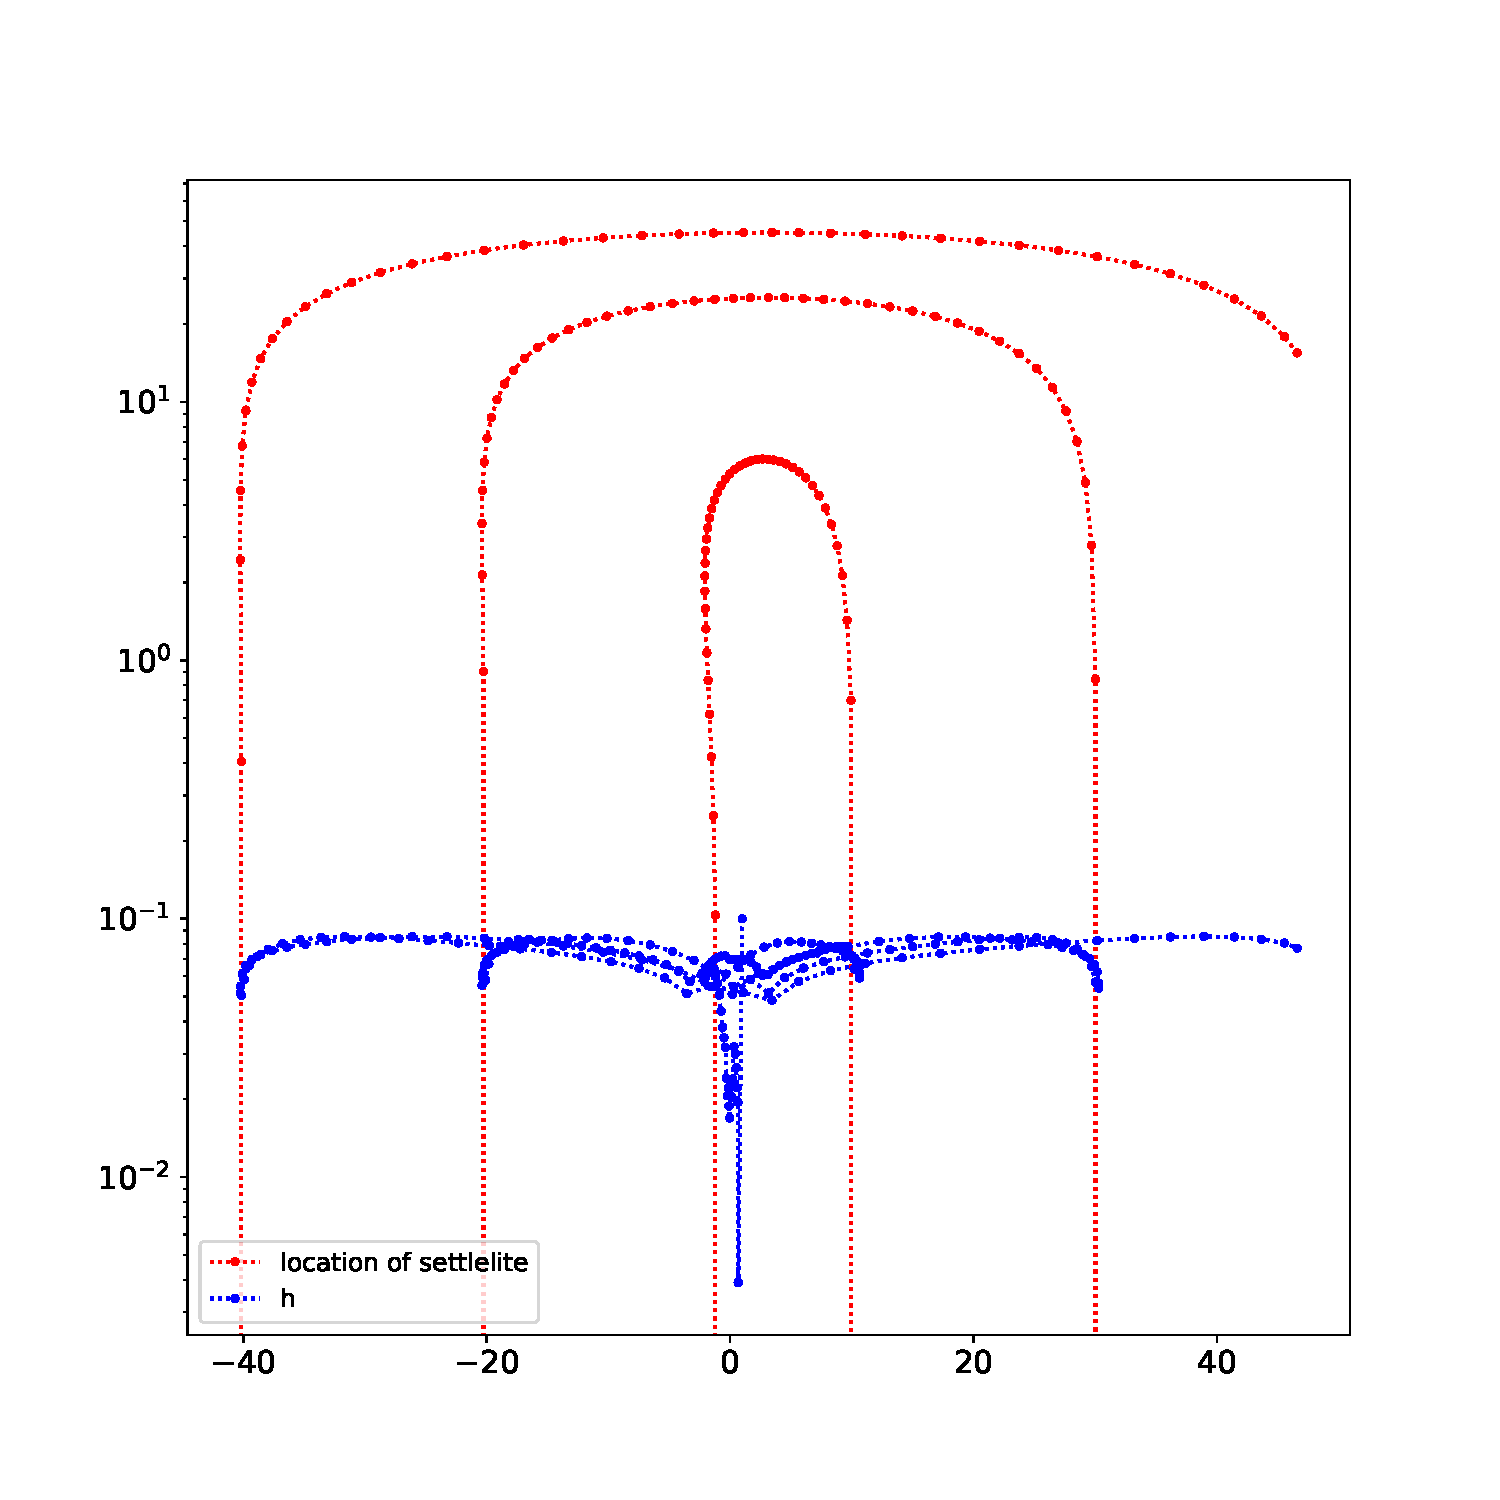
\includegraphics[width=1\textwidth]{xandhs.pdf}
  \caption{Location settlelite and Stepsize}
\end{figure}

이를 조금 더 작은 단위로 확인하기 위해, List Slicing을 이용하여 보면 조금 흥미로운 현상을 볼 수 있는데, 바로 위성의 기울기에 따라 영향을 받는 것을 볼 수 있다. 좀전에, 적응형 단계 크기 제어 방법을 사용하는 것은 도함수의 크기에 큰 차이가 있을 때 특히 중요하다라고 적혀있었는데, 이는 기울기의 큰 변화가 존재할때, h또한 매우 커지는 것을 볼 수 있다. 이를 좀더 파악하기 위해서 몇가지 그림을 확인하면 다음과 같다. 다음 그림은 log계수가 아닌 실제 값을 y축으로 설정한 그래프이다.

\begin{figure}[!ht]
  \centering
  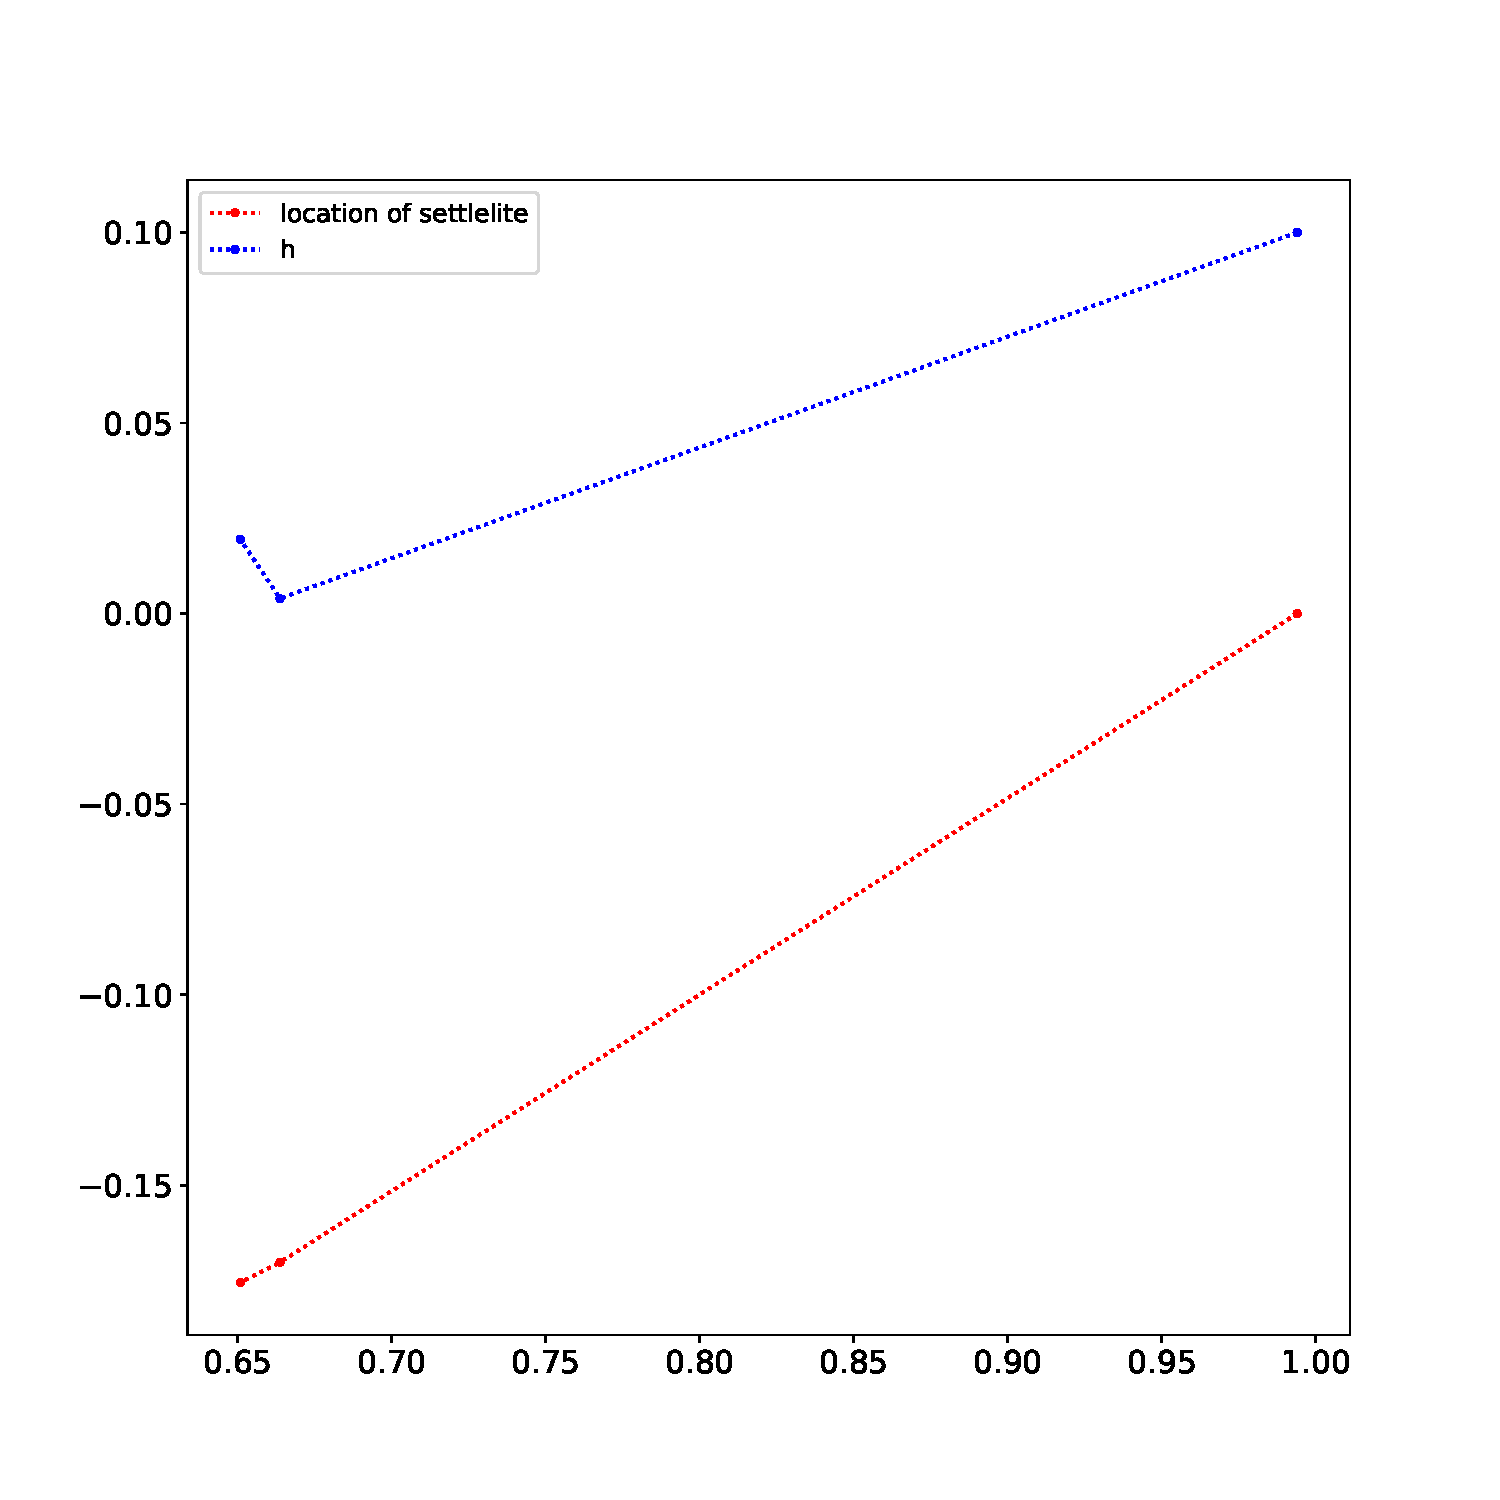
\includegraphics[width=0.8\textwidth]{xandhs2.pdf}
  \caption{[xlist[:-230], and ylist[:-230}
\end{figure} 
  
\begin{figure}[!ht]
  \centering
  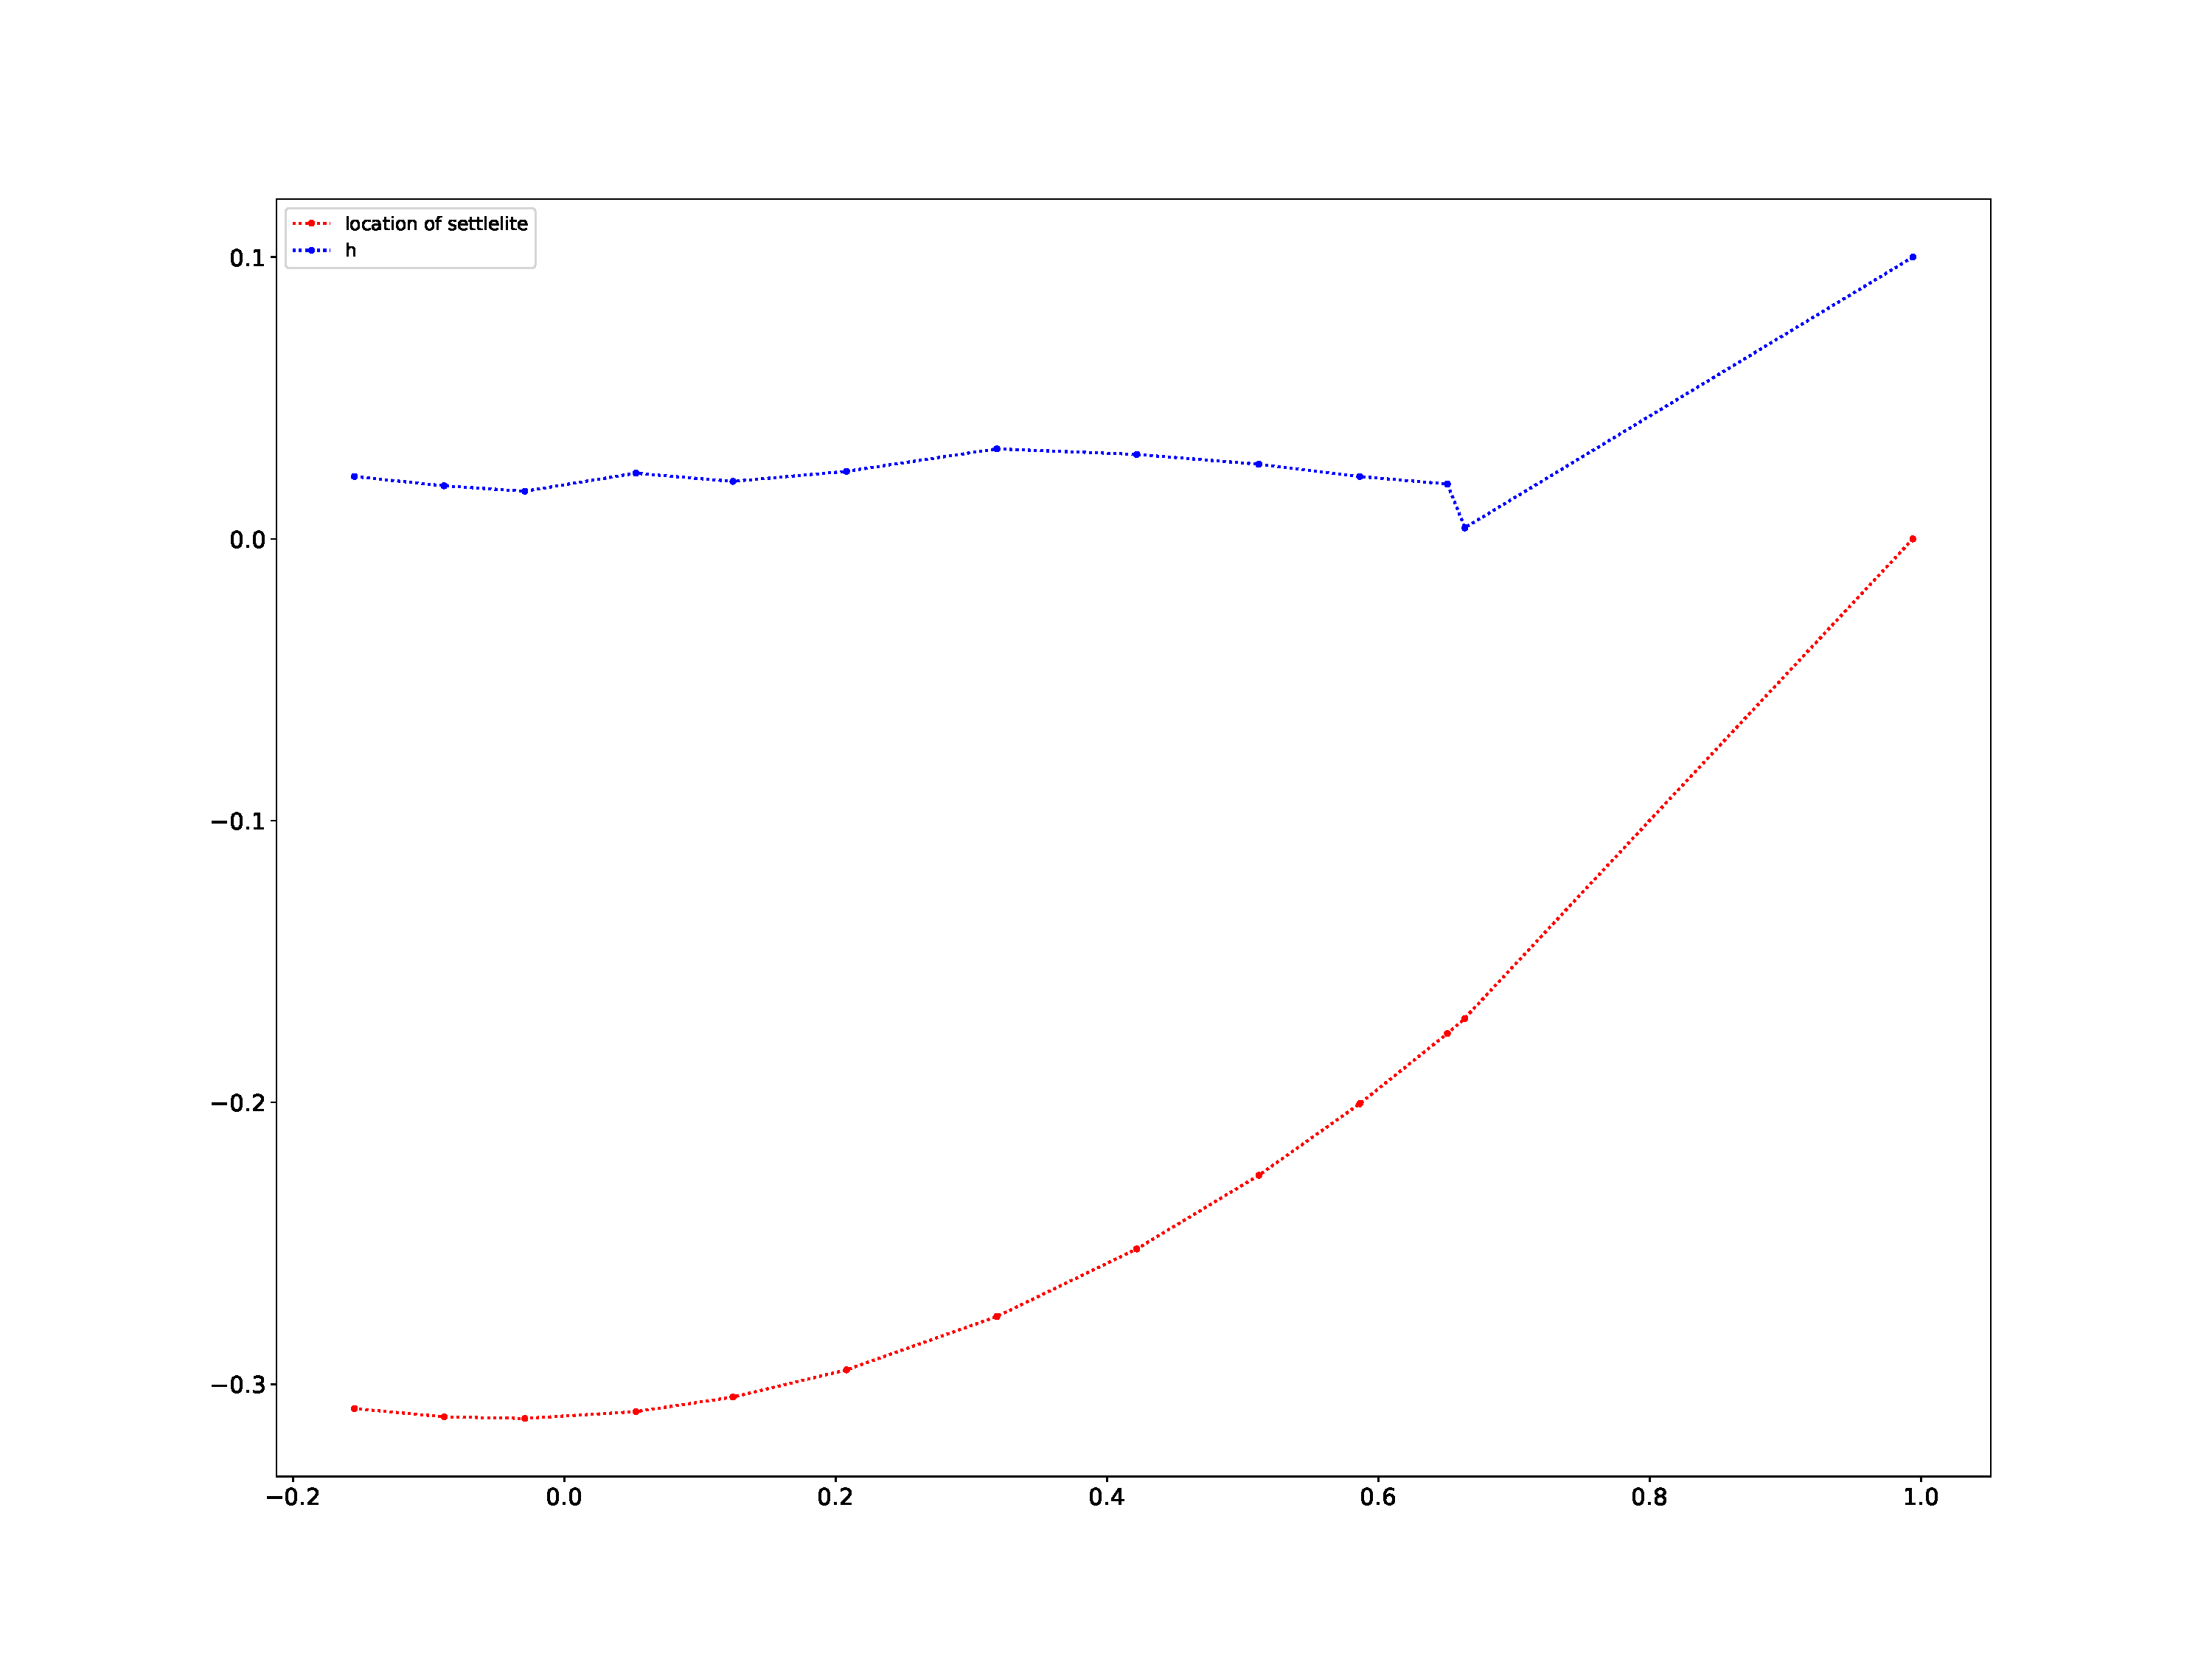
\includegraphics[width=0.8\textwidth]{xandhs3.pdf}
  \caption{[xlist[:-220], and ylist[:-220}
\end{figure} 

\begin{figure}[!ht]
  \centering
  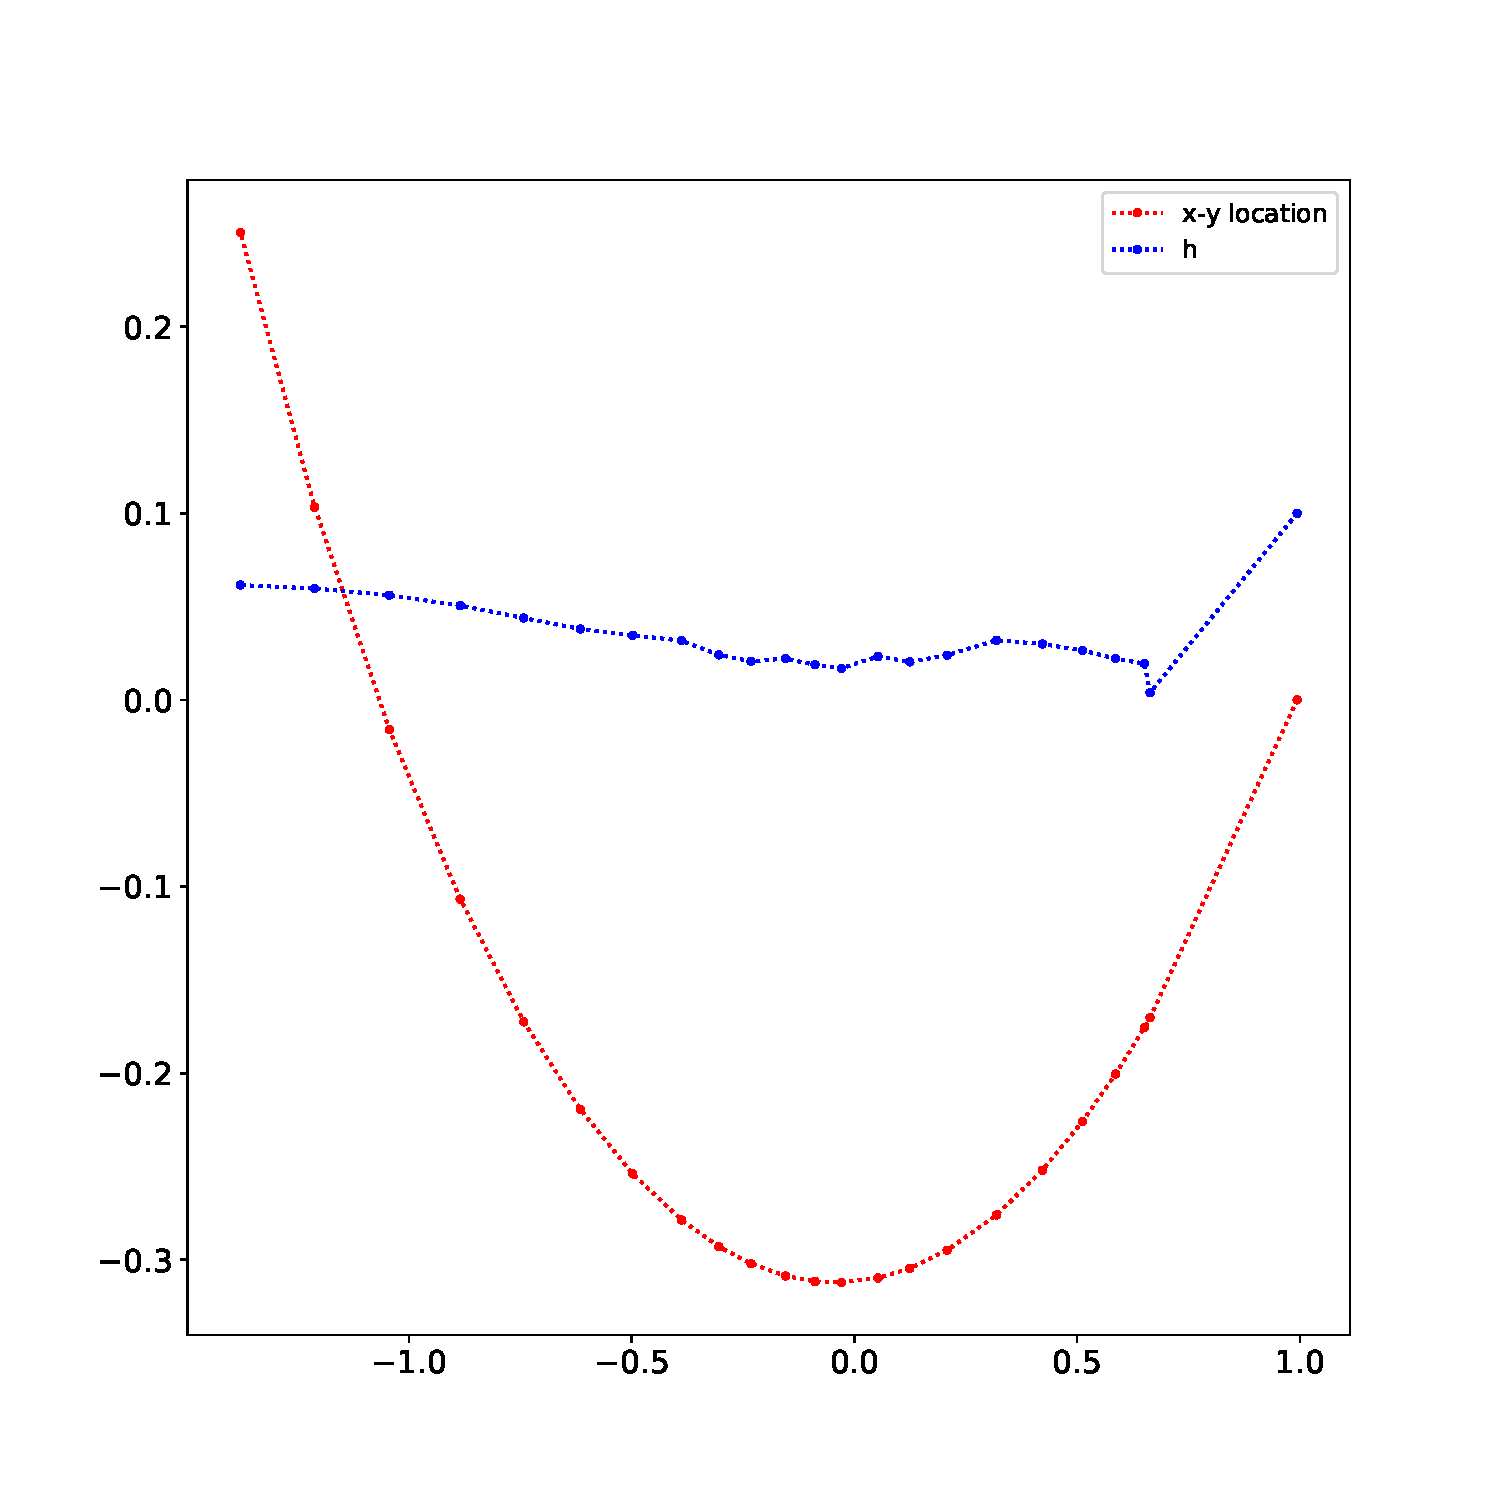
\includegraphics[width=0.8\textwidth]{xandhs4.pdf}
  \caption{[xlist[:-210], and ylist[:-210}
\end{figure} 

기울기와 h사이의 관계를 그래프로 그려보면 다음과 같다.
\begin{lstlisting}[language=Python]
h_list = hs 
ylist_list = ylist 
xlist_list = xlist

xlist_2 = xlist_list[2:] 
xlist_2 = np.append(xlist_2, xlist_list[-1]) 
diff_xlist_err = []

ylist_2 = ylist_list[2:] 
ylist_2 = np.append(ylist_2, ylist_list[-1]) 
diff_ylist_err = []
a = 0
b = 220

for i, j in zip(ylist_2, ylist_list[1:]):
    diff_xlist_err.append(abs(i - j))

for i, j in zip(xlist_2, xlist_list[1:]):
    diff_ylist_err.append(abs(i - j))

grad = []
for i, j in zip(diff_xlist_err, diff_ylist_err):
    grad.append(abs(i / j))
    
for i, j in zip(h_list_2, h_list):
    diff_h_list.append(i - j)
    

rel_err_2 = rel_err_list[2:] 
rel_err_2.append(rel_err_list[-1]) 
diff_rel_err = []

for i, j in zip(rel_err_2, rel_err_list[1:]):
    diff_rel_err.append(i - j)

    
#Plotting (x, y)!!
plt.figure(figsize=[10, 10])
plt.semilogy(xlist[a:b], grad[a:b], ".:r",xlist[a:b], rel_err_list[a:b], ".:b")


plt.grid()
plt.xlabel("$x$")
plt.ylabel("$\delta$")
#plt.title("h & rel_{err} Graph")
plt.legend(["$gradient$", "h"], fontsize=12)
plt.tight_layout()
plt.show()
\end{lstlisting}


\begin{figure}[!ht]
  \centering
  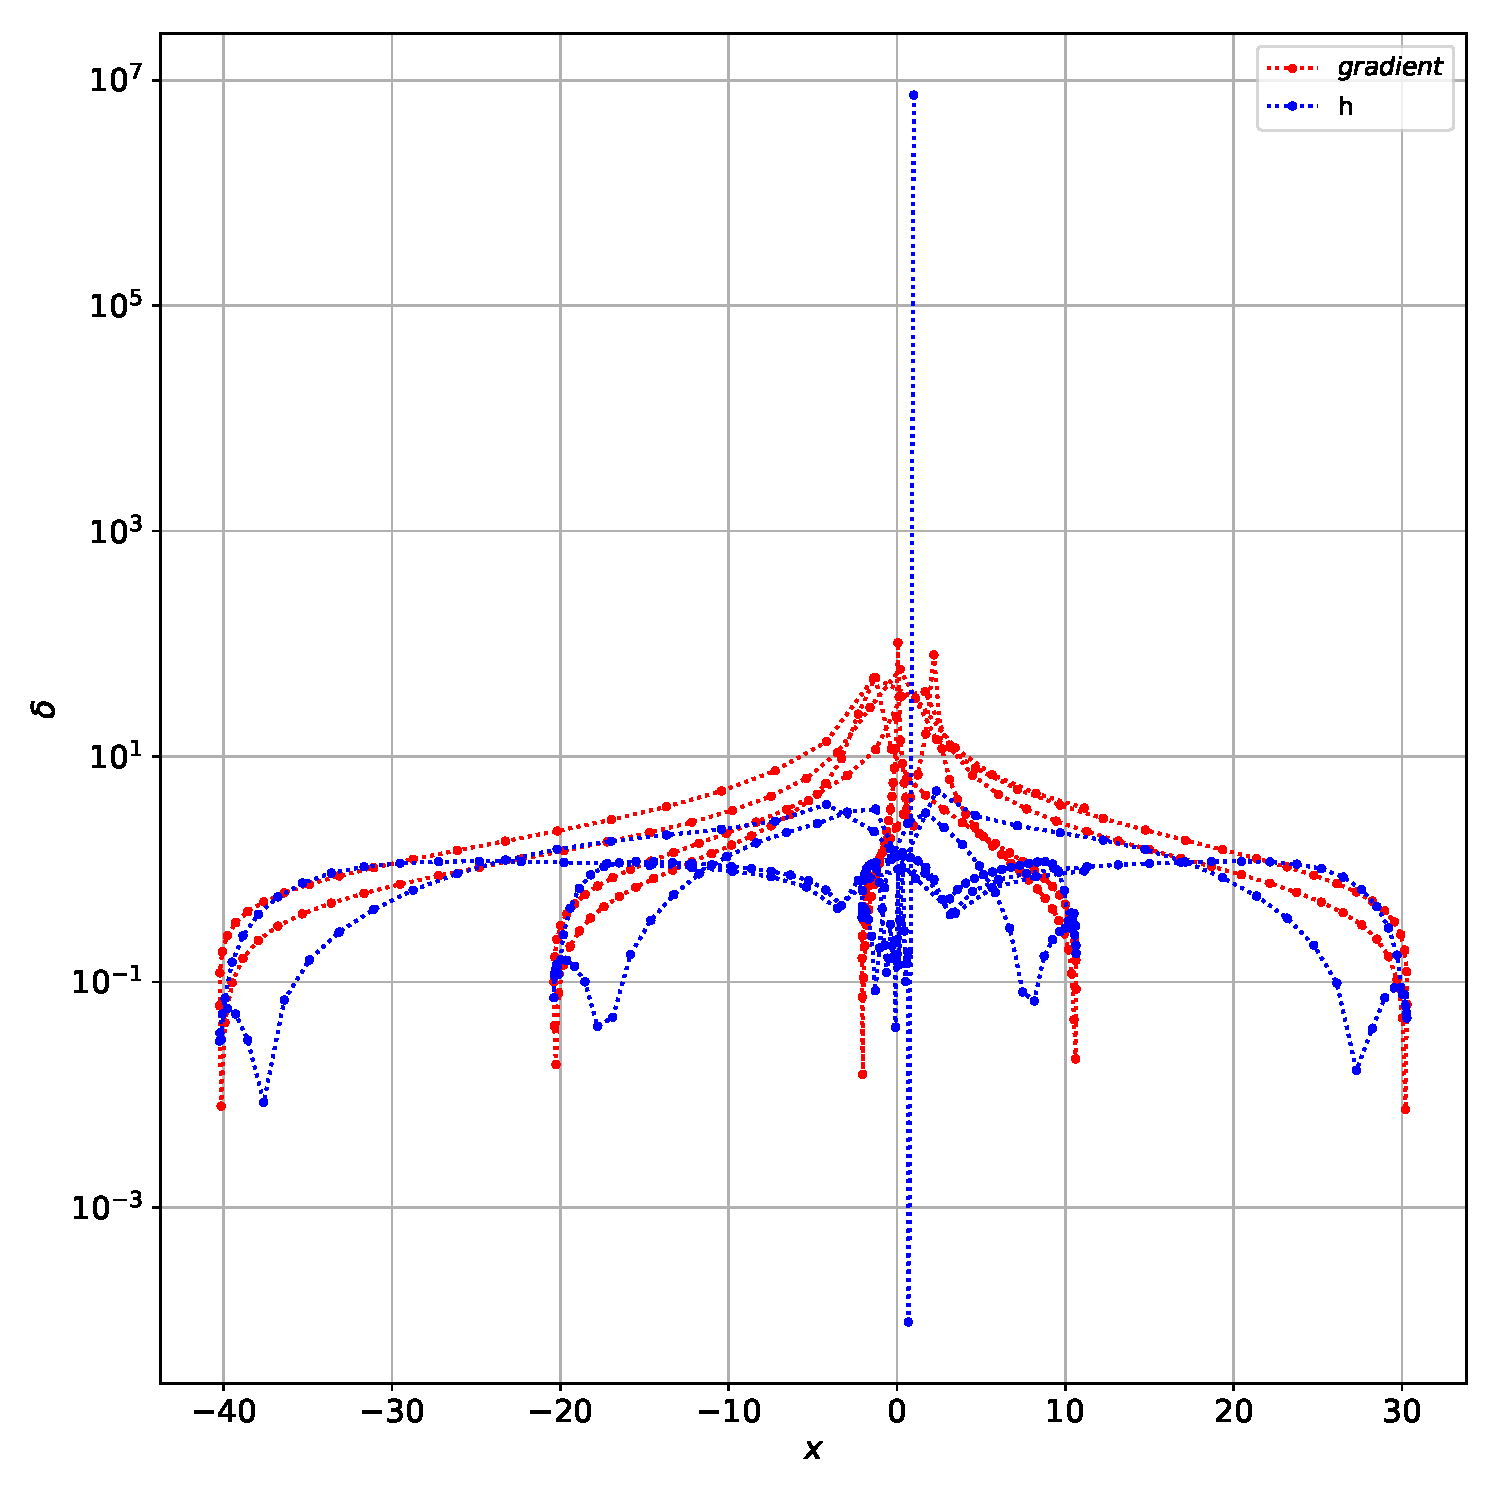
\includegraphics[width=0.8\textwidth]{xandhs5.pdf}
  \caption{gradient and h, [0: 220}
\end{figure} 
Stepsize h의 변화를 이해하기 위해서 Adaptive Stepsize Control의 개념을 다시보면, h의 변화는 

\begin{equation}
h \rightarrow 0.9\times h\times \min \left(\max \left(\left({\frac{\text{tol}}{2\left|\tau_{n+1}^{(1)}\right|}}\right)^{1/2},0.3\right),2\right)
\end{equation}
에 의해 조정되는 것을 알 수 있다. 그리고 이것을 구현한 예시코드(embedded rk4 ode)에서 쓰인 코드를 다시 주목하면,

\begin{lstlisting}[language=Python]
delta = d1*k1 + d2*k2 + d3*k3 + d4*k4 + d5*k5 + d6*k6
y_tmp = abs(y) + abs(h*k1) 
desired = abs(abstol) + abs(y_tmp*reltol)
rel_err = delta / desired
        
h = h / max(abs(rel_err)**0.2, 1e-2)    # limit the max stepsize increase
h = min(max(h, hminmax[0]), hminmax[1]) # finally, clamp stepsize
\end{lstlisting}
이는 위에 Adaptive Stepsize Control 에서 소개된 아래의 식을 적용한 부분이다.

\begin{equation}
\Delta \equiv y_{n + 1} - y_{n + 1}^* = \sum_{i = 1}^{6} \left(c_i - c_i^*\right) k_i
\end{equation}
이 부분이 곧, rel err의 delta에 해당하는 부분이고, 이는 분자이다. 그리고 분모 부분은 desired로, 위의 식

\begin{equation}
h_0 = h_1 \left| \frac{\Delta_0}{\Delta_1} \right|^{0.2}
\end{equation}
가 적용된 부분이다. 우리가 주목해야 할 점은 코드 1~3줄에 의해 Stepsize h는 rel err에 의해서 적용되고 rel err은 delta와 desired로 결정된다는 것이다. 또한, 그래프에서 볼 수 있는 급격한 변화는코드 6~8줄에서 h의 최소와 최댓값을 제한했고, stepsize가 갑자기 커지는 것을 막기 위해 max함수로 제한을 걸었기 때문에 발생한 경우라는 것도 알 수 있다. 또한 이것을 수식적으로 이해하기 위해 초기값 h = 0.1을 넣었을때를 고려해보면 쉽게 이해할 수 있는데, reltol과 abstol에 따라 분모가 작아지게 되면서 rel err값이 증가하게 되지만, h는 제한이 있기 때문에 h값의 제한에 다다를 경우 h가 제한 값을 선택하면서 급변하게 되는 현상이다. 이러한 부분은 Figure 14에서 볼 수 있듯이, 0.1에서 0.6로 갈때 부자연스럽게 빠르게 꺾이는 부분에서 확인할 수 있다.

하지만 그외에도 크게 변화하는 부분을 그래프에서 볼 수 있었는데, 바로 이 부분이 도함수 크기가 크게 변화하는 부분이 존재했을 경우이다. 또는 부호가 갑자기 달라지는 경우, Stepsize h와 Gradient 사이의 그래프에서 볼 수 있듯이 급격한 변화를 보이는 것을 볼 수 있다. 이렇게 Stepsize h가 기울기와 연관이 있는 이유는 바로 Runge-Kutta 방법을 적용했을때에 정의한 rel err의 값 때문이다. 이는 아래에서 더 설명할 것이다. 우선 h가 작으면 rel err이 작아지게 되고 그러면 h는 증가값을 가지면서 다음 Step에서는 rel err은 커지게 된다. 하지만 rel err값이 다시 커지면 h가 작아지게 되면서 서로의 값을 따라가게 되는데, 그 기준으로 영향을 미치는 값은 그 함수의 값이다. 왜냐하면, 식에서 쓰인 K1 K2 들의 영향을 받으면서, 생기는 현상인데, function에 해당하는 값이 부호가 변할때나 급증할때, rel err값또한 변화폭이 강해지므로 함수의 변화의 정도에 따라 결정되는 모습을 볼 수 있고 결론적으로는 함수와 비슷한 모양을 따라가는 것을 확인할 수 있다. 

\pagebreak































\section{Dipole Field Line Tracing}
\subsection{Problem Recognition} 
지구 자기장의 쌍극자 모델은 실제 지구 자기장의 1차 근사치이다. 
\begin{figure}[!ht]
  \centering
  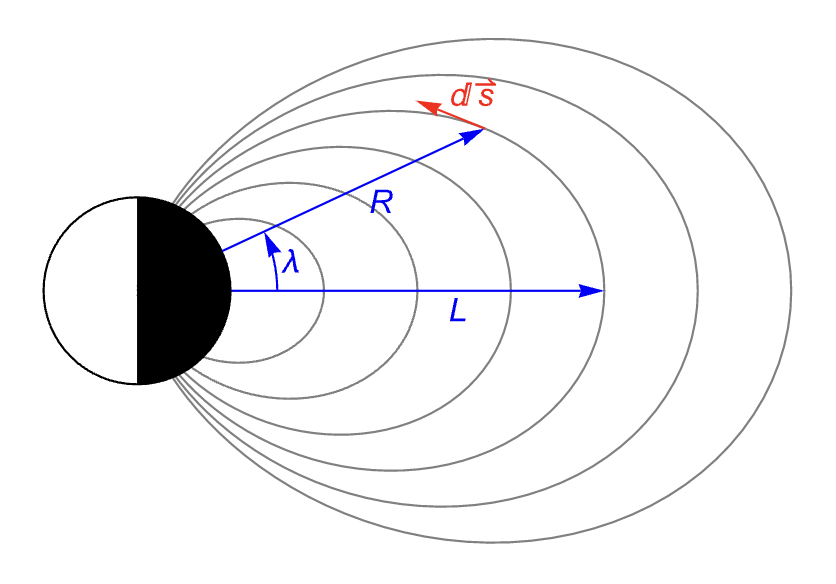
\includegraphics[width=0.8\textwidth]{ElectricField.png}
  \caption{dipole model of the Earth’s magnetic field}
\end{figure} 
2차원 자오면을 고려할 때 radial과 latitudinal field는 다음과 같이 설명된다.
\begin{equation}
\begin{split}
\begin{aligned}
B_r &= -2 \frac{B_0}{R^3} \sin\lambda \\
B_\lambda &= \frac{B_0}{R^3} \cos\lambda \\
\end{aligned}
,
\end{split}
\end{equation}
여기서 $R = r / R_E$이고, $B_0 = 3.12 \times 10^{-5}\ \mathrm{T}$ 이다. 이때 단위벡터는 
\begin{equation}
\begin{split}
\begin{aligned}
\hat{\mathbf e}_r &= \cos\lambda \hat{\mathbf x} + \sin\lambda \hat{\mathbf x} \\
\hat{\mathbf e}_\lambda &= -\sin\lambda \hat{\mathbf x} + \cos\lambda \hat{\mathbf x} \\
\end{aligned}
,
\end{split}
\end{equation}
이고, 자기장 벡터는 다음과 같다.
\begin{equation}
\mathbf B = B_r \hat{\mathbf e}_r + B_\lambda \hat{\mathbf e}_\lambda
.
\end{equation}
이때, 변위 벡터를 $\mathbf B$라고 하고 자기장선은 미분 방정식을 적분하여 그릴 수 있다.
\begin{equation}
d\mathbf s = \frac{\mathbf B}{|\mathbf B|} dt
\end{equation}
여기서 t는 경로 매개변수이다. 이 문제는 마찬가지로 미분 방정식을 적절하게 정의하여 위의 그림과 같은 자기장선을 그려야 한다.

\subsection{Development of a solution} 
먼저 우리는 자기장 선을 그리고, 그 위에 지구 모형의 원을 원점에 넣어서 그래프를 그려줄 것이다. 먼저 식을 확인하면, 기존에 풀었던 방식과 다르게 x, y로 이루어진 데카르트 좌표계가 아닌, radial과 latitudinal 로 이루어진 좌표계이다. 따라서 이 문제를 접근하려면 우선 위에서 제시된 radial-latitudinal 좌표계로 만들어 미분방정식을 풀어준 뒤, 구한 radil-latitudinal 좌표값들을  x-y 로 이루어진 좌표계로 변환하여 그래프를 그리면 된다. 따라서 우리는 Y를  ($r$, $\lambda$)로 잡는다.

\begin{equation}
(B_{r}, B_{\lambda}) = \left (  \frac{-2B_{0}}{R^3}sin\lambda  + \frac{B_{0}}{3}cos\lambda \right ) 
\end{equation}
이기 때문에, 이를 $\mathbf B$과 비교하면, 식 55를 통해, $|\mathbf B|$ 값을 $(B_{r}, B_{\lambda})$에 각각 나누어줌으로써, 우리가 구하고자 하는 $\frac{dt}{ds}$ 꼴의 형태를 구할 수 있다.  이것을 코드로 구현하면 다음과 같다.

\begin{lstlisting}[language=Python]
def F_B(t, Y):
    [r, lamb] = Y
    R = r / R_E
    B_r = -2 * (B_0 / R**3) * np.sin(lamb)
    B_lambda = B_0 / 3 * np.cos(lamb)
    dY = [(B_r) / (B_r**2 + B_lambda**2)**0.5, (B_lambda) / (B_r**2 + B_lambda**2)**0.5]
    return np.array(dY) # (B_r, B_lambda)
\end{lstlisting}
그러면 우리는 Function에 대한 정의가 끝나게 된다. 우리는 앞서서 좌표계가 다른 것을 인지하고 있기 때문에, 후속처리로 좌표계를 변환시키는 작업을 해야 한다. 이와 같은 작업은 다음 함수를 통해서 쉽게 바꿀 수 있다. 

\begin{lstlisting}[language=Python]
def pol2cart(rho, phi):
    x = rho * np.cos(phi)
    y = rho * np.sin(phi)
    return (x, y)
\end{lstlisting}
따라서, 식
\begin{equation}
\mathbf B = B_r \hat{\mathbf e}_r + B_\lambda \hat{\mathbf e}_\lambda = \frac{-2B_{0}}{R^3}sin\lambda \hat{\mathbf e}_r  + \frac{B_{0}}{3}cos\lambda \hat{\mathbf e}_\lambda
\end{equation}
처럼 우리가 구해준 radil-latitudinal 좌표계의 solution을 각각 x1, y1의 변수에 저장한 후, 그것을 pol2cart 함수에 대입하여, x-y좌표계에서의 좌표값을 구해준다. 그리고 구한 x-y좌표값으로 그래프를 그리면 우리가 구하고자 하는 ($r$, $\lambda$)의 그래프를 x-y좌표계에서 그릴 수 있게 된다. 편의상, 지구의 반지름을 1로 두고, hinit을 0.001로 두고 문제를 풀어보았다. 또한, abstol값과 reltol 모두 $10^{-11}$으로 정했고, iterations의 한계값은 10000으로 정한다. 그것을 나타낸 코드가 다음과 같다.

\begin{lstlisting}[language=Python]
#constant

B_0 = 3.12 * 1e-5 #T

def F_B(t, Y):
    [r, lamb] = Y
    R = r / R_E
    B_r = -2 * (B_0 / R**3) * np.sin(lamb)
    B_lambda = B_0 / 3 * np.cos(lamb)
    dY = [(B_r) / (B_r**2 + B_lambda**2)**0.5, (B_lambda) / (B_r**2 + B_lambda**2)**0.5]
    return np.array(dY) # (B_r, B_lambda)
    
def pol2cart(rho, phi):
    x = rho * np.cos(phi)
    y = rho * np.sin(phi)
    return (x, y)
#1
R_E = 1
hinit = 0.001
xlim = 0, 20 *np.pi
Yinit   = np.array([-0.225, 300]) # 25 5000

t, Y, h = embedded_rk4_ode(F_B, Yinit, hinit, xlim, abstol=1e-11, reltol=1e-11,
                           hminmax=(1e-11, 10), max_iterations=10000)
x1, y1 = map(np.array, zip(*Y))

# drawing
plt.figure(figsize=[20, 20])
plt.plot(pol2cart(x1, y1)[0], pol2cart(x1, y1)[1],'.:k',label="$Dipole Field Line$")

       #pol2cart(x7, y7)[0], pol2cart(x7, y7)[1],'.:k',

plt.plot(0,0, 'ob', ms=100)
plt.plot(0,0, 'ob', ms=10, label="$Earth$")
#plt.plot(pol2cart(x,y)[0], pol2cart(x,y)[1], '-b')
plt.legend(loc='best', ncol=2, fontsize=14)
plt.savefig("Electric.pdf")

\end{lstlisting}

\begin{figure}[!ht]
  \centering
  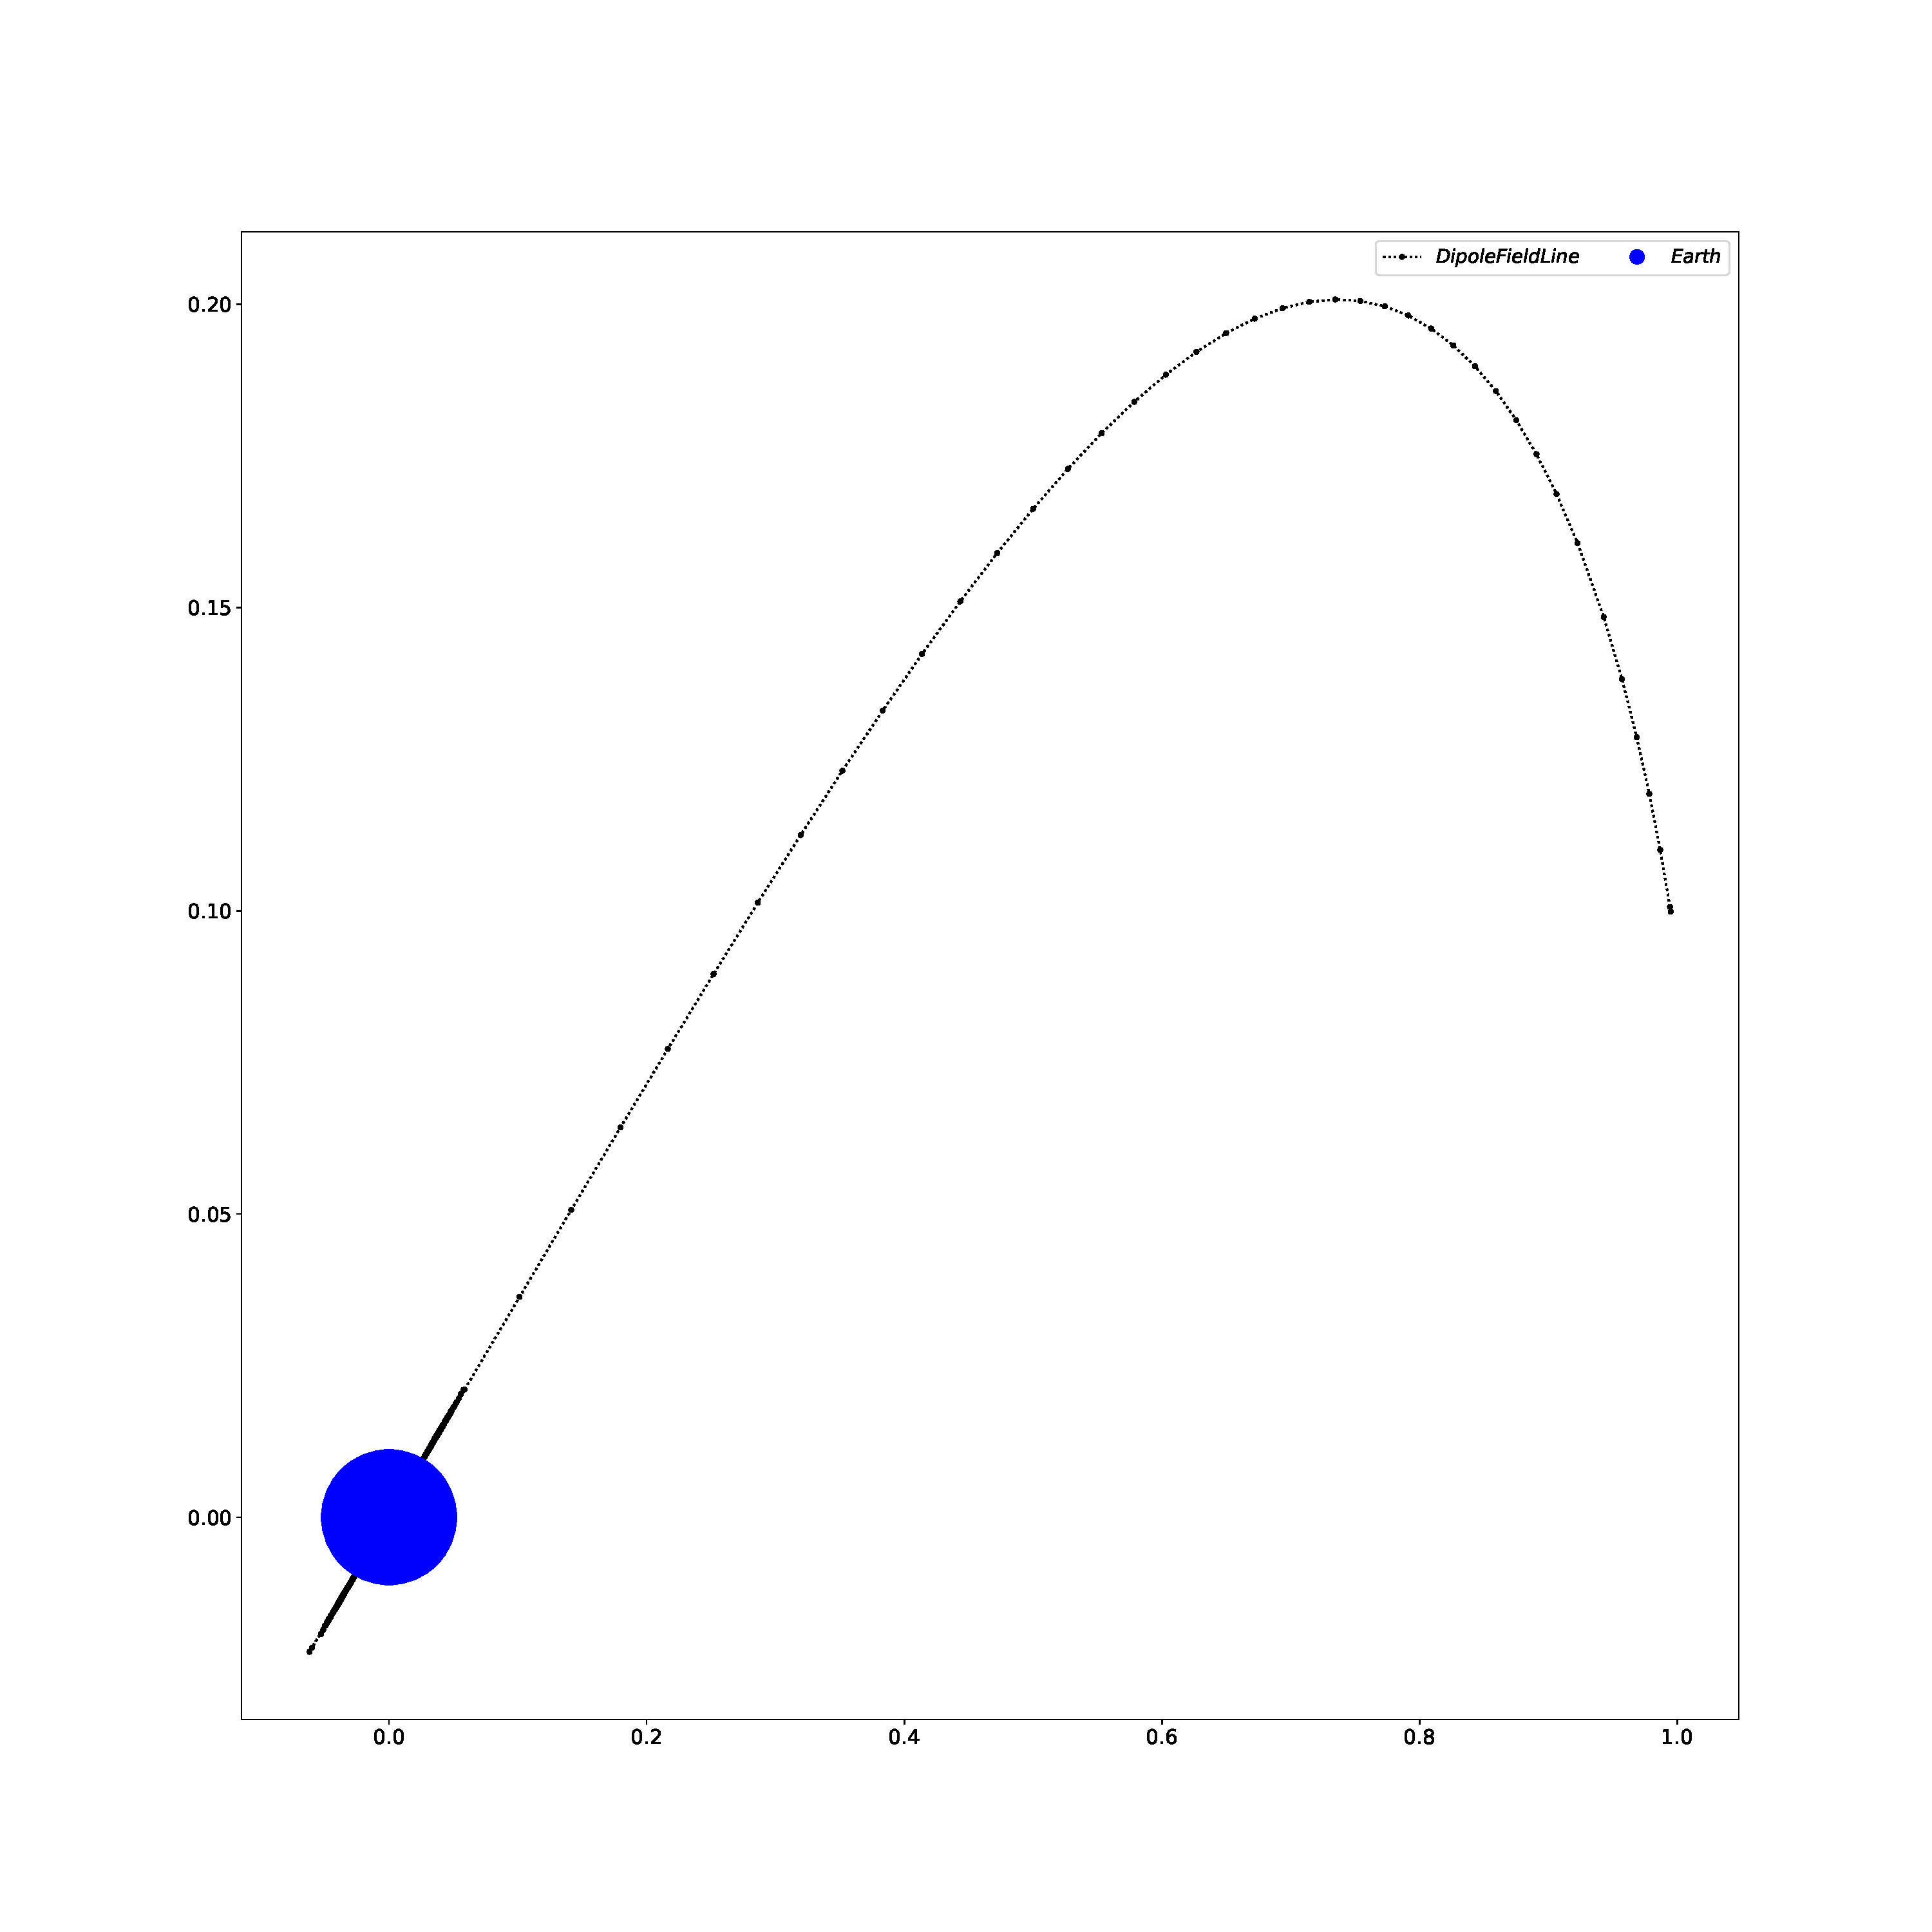
\includegraphics[width=0.8\textwidth]{Electric.pdf}
  \caption{Dipole Field Line Tracing One line}
\end{figure} 
하지만 이렇게 그래프를 완성하게 되면 오직 하나의 자기장선만이 그려지게 되는데, 이 이유는 초기값을 Yinit   = np.array([-0.225, 300])로 정했기 때문이다. 앞에서 예제들과 같이, 초기값을 어떻게 선정하느냐에 따라서 만드는 x-y의 자취가 달라지므로, 초기값을 적절하게 선택하여 우리가 원하는 그래프를 그리는 방식을 Shooting Method를 인용할 것이다.

계속해서 우리가 원하는 그래프를 가지는 초기값을 찾기위해 반복적으로 함수를 실행했고, 마침내 적절한 초기값 [-0.225, 300], [-0.223, 350], [0.225, 30], [0.224, 3071], [0.21, 200], [-0.22, 4000] 을 넣었을때, 우리가 원하는 지구 자기장선의 모습을 볼 수 있었다. 그래프를 중복하여 그려야했기 때문에, 다른 값들은 조정하지 않으며 오직 초기값만 수정하여 그래프를 그리게 되면, 다음과 같다.

\begin{lstlisting}[language=Python]
#1
R_E = 1
hinit = 0.001
xlim = 0, 20 *np.pi
Yinit   = np.array([-0.225, 300]) # 25 5000

t, Y, h = embedded_rk4_ode(F_B, Yinit, hinit, xlim, abstol=1e-11, reltol=1e-11,
                           hminmax=(1e-11, 10), max_iterations=10000)
x1, y1 = map(np.array, zip(*Y))

#2
R_E = 1
hinit = 0.001
xlim = 0, 20 *np.pi
Yinit   = np.array([-0.223, 350]) #4
t, Y, h = embedded_rk4_ode(F_B, Yinit, hinit, xlim, abstol=1e-11, reltol=1e-11,
                           hminmax=(1e-11, 10), max_iterations=10000)
x2, y2 = map(np.array, zip(*Y))

#3
R_E = 1
hinit = 0.001
xlim = 0, 20 *np.pi
Yinit   = np.array([0.225, 30]) 
t, Y, h = embedded_rk4_ode(F_B, Yinit, hinit, xlim, abstol=1e-11, reltol=1e-11,
                           hminmax=(1e-11, 10), max_iterations=100000)
x3, y3 = map(np.array, zip(*Y))

#4
R_E = 1
hinit = 0.001
xlim = 0, 20 *np.pi
Yinit   = np.array([0.224, 3071]) #4
t, Y, h = embedded_rk4_ode(F_B, Yinit, hinit, xlim, abstol=1e-11, reltol=1e-11,
                           hminmax=(1e-11, 10), max_iterations=10000)
x4, y4 = map(np.array, zip(*Y))

#5
R_E = 1
hinit = 0.001
xlim = 0, 20 *np.pi
Yinit   = np.array([0.21, 200]) #4
t, Y, h = embedded_rk4_ode(F_B, Yinit, hinit, xlim, abstol=1e-11, reltol=1e-11,
                           hminmax=(1e-11, 10), max_iterations=10000)
x5, y5 = map(np.array, zip(*Y))

#6
R_E = 1
hinit = 0.001
xlim = 0, 20 *np.pi
Yinit   = np.array([-0.22, 4000]) #4
t, Y, h = embedded_rk4_ode(F_B, Yinit, hinit, xlim, abstol=1e-11, reltol=1e-11,
                           hminmax=(1e-11, 10), max_iterations=10000)
x6, y6 = map(np.array, zip(*Y))

# drawing
plt.figure(figsize=[15, 15])
plt.plot(pol2cart(x1, y1)[0], pol2cart(x1, y1)[1],'.:k',
       pol2cart(x2, y2)[0], pol2cart(x2, y2)[1],'.:k',
        pol2cart(x3, y3)[0], pol2cart(x3, y3)[1],'.:k',
        pol2cart(x4, y4)[0], pol2cart(x4, y4)[1],'.:k',
        pol2cart(x5, y5)[0], pol2cart(x5, y5)[1],'.:k',
        pol2cart(x6, y6)[0], pol2cart(x6, y6)[1],'.:k',
        )
plt.plot(0,0, 'ob', ms=100, label="$m_1$")
plt.savefig("Electric2.pdf")
\end{lstlisting}

\begin{figure}[!ht]
  \centering
  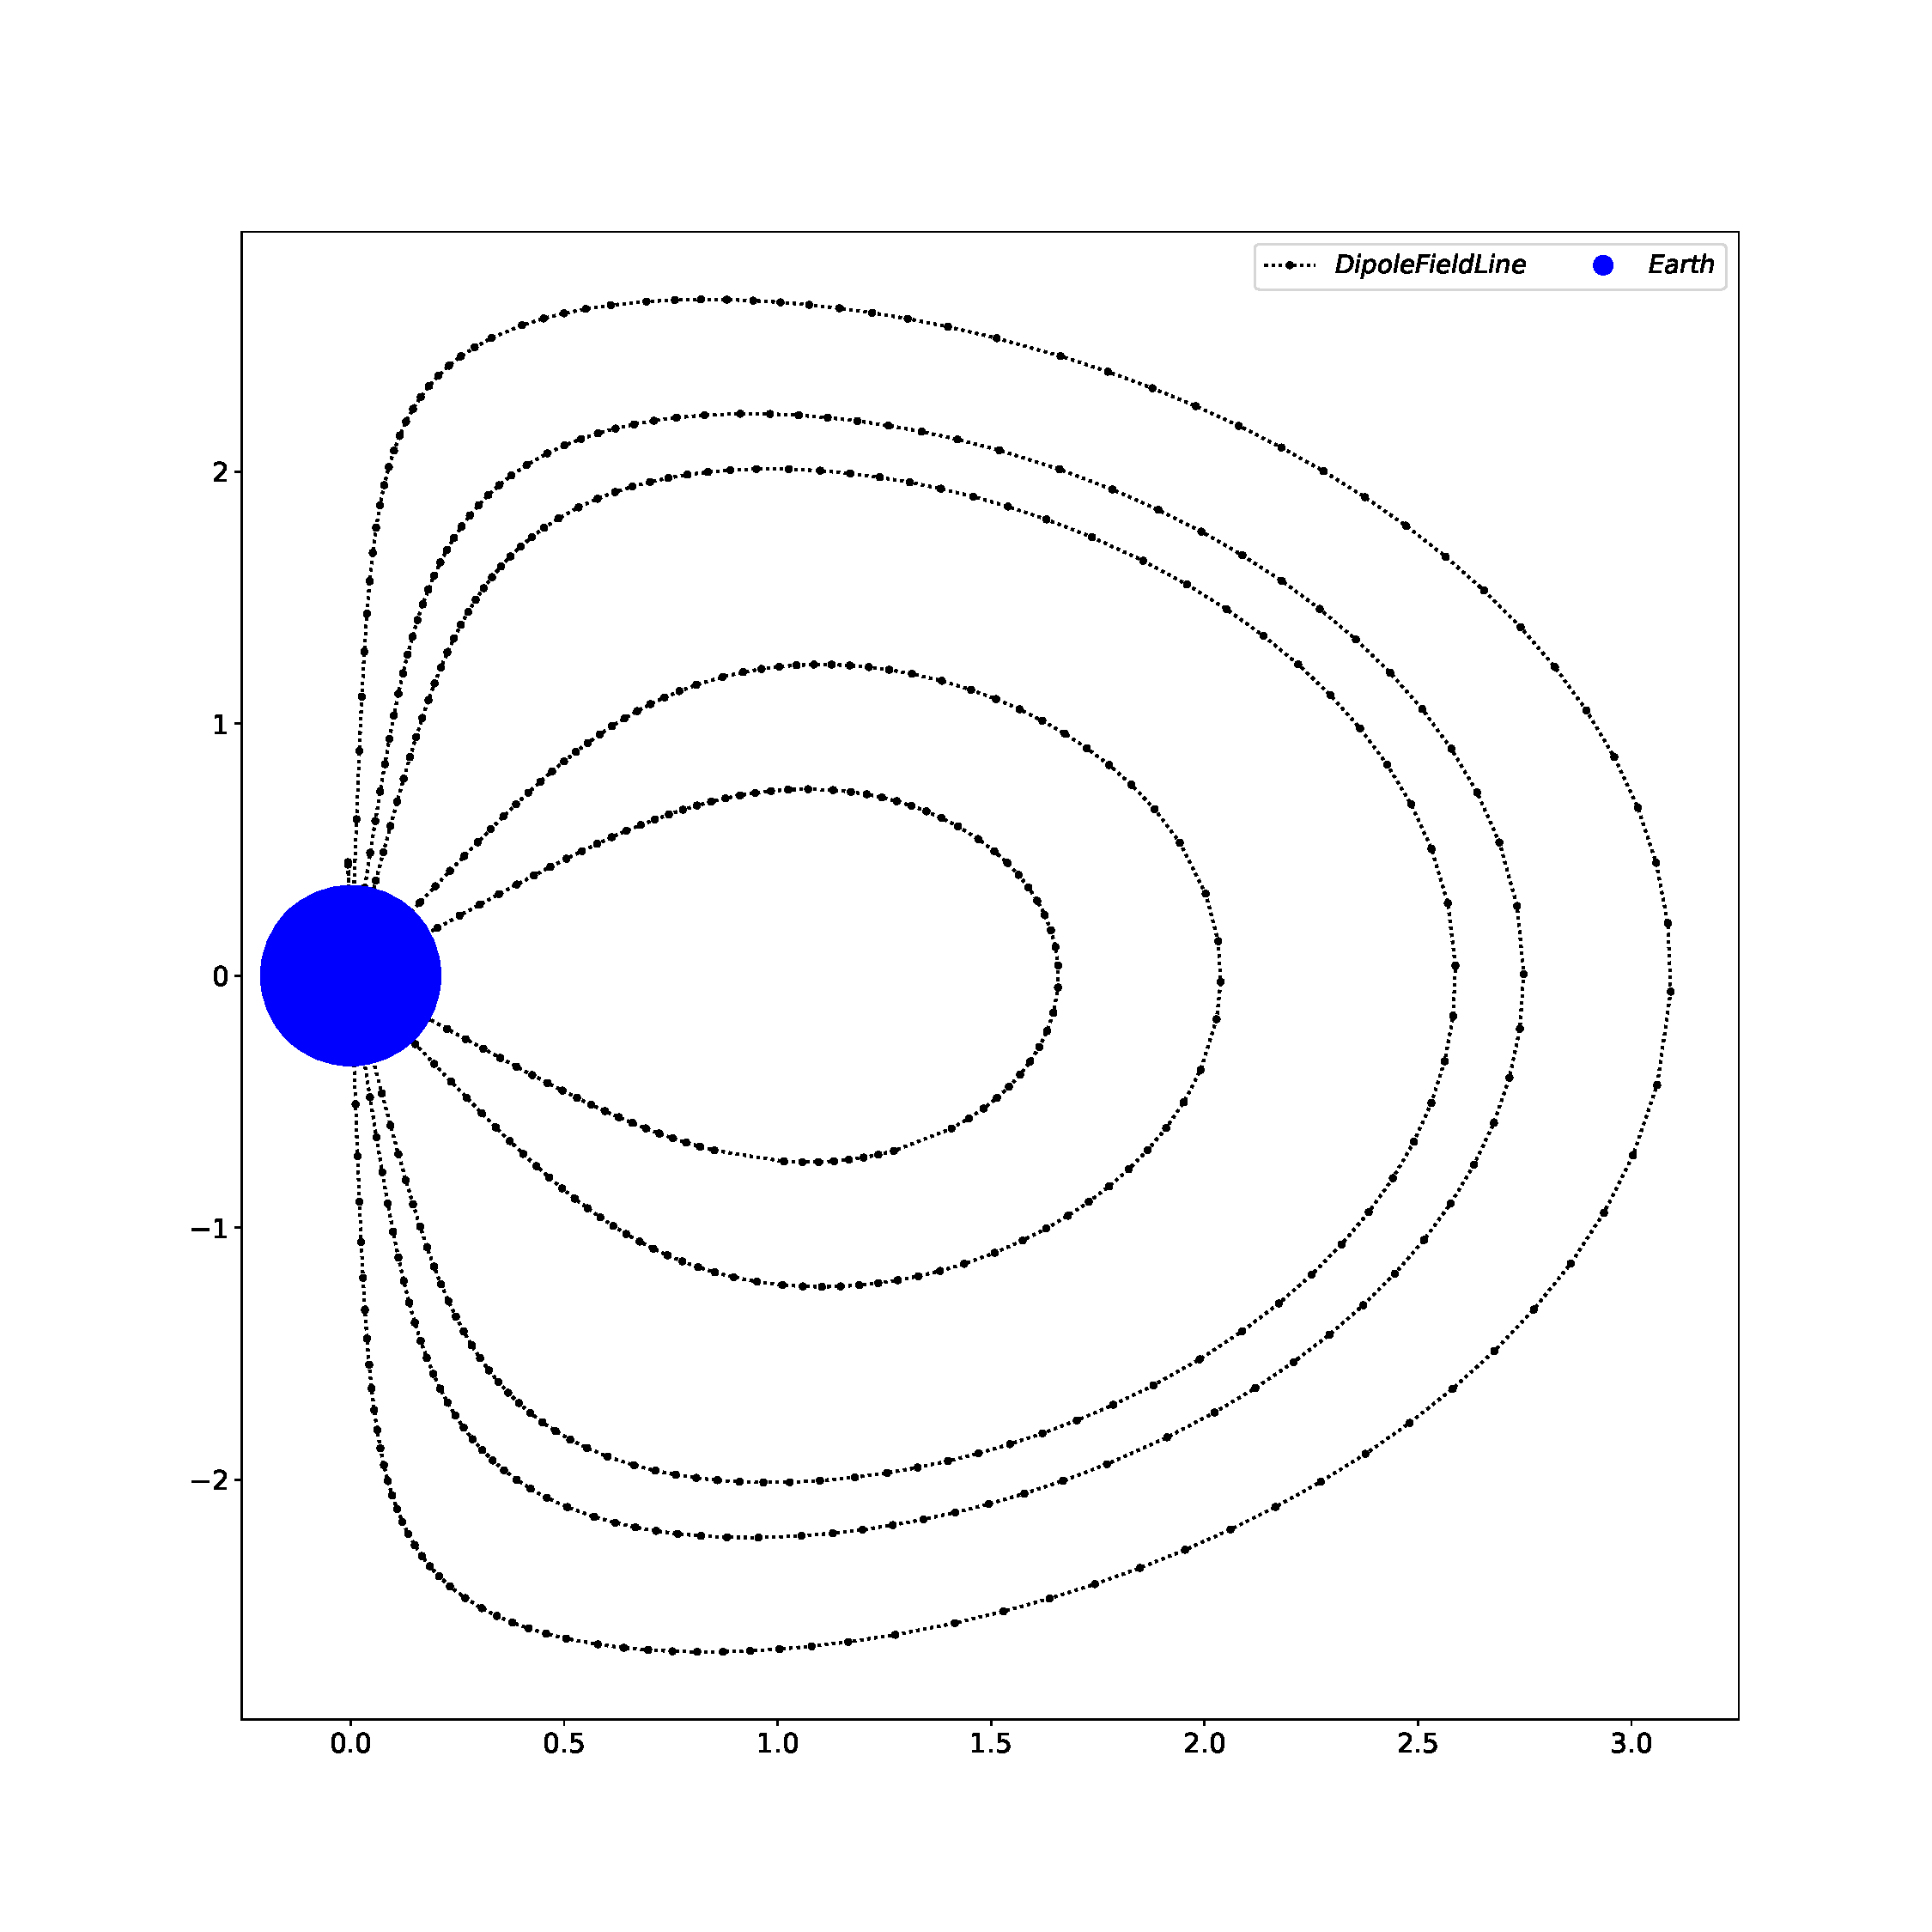
\includegraphics[width=0.8\textwidth]{Electric2.pdf}
  \caption{Dipole Field Line Tracing Six Line}
\end{figure} 
이 그래프는 적절한 초기값을 가지지 못하면, 자기장선이 적합하게 그려지지 않는다. 따라서 반복적으로 우리가 원하는 초기값을 얻기 위해서 함수를 반복시켜야 했다. 

상미분 방정식을 푸는 방식에 초기값을 이용하면, 근사적으로 적은 정보만으로 훌륭한 근사치를 뽑을 수 있지만, 초기값에 따라서 결과값이 크게 변할 수 있는 점을 주목할 수 있다. 또한, 전에 다뤘던 방식과 달리, Stepsize h를 함수의 도함수와의 관계로 엮어, 함수가 급격하게 증가하는 경우 계산처리를 해야할 경우가 매우 커질 수 있지만 그럼에도 불구하고 Stepsize가 우리가 정한 범위 내에서 조정되면서 효율적인 계산을 할 수 있다는 점을 알 수 있었다.
\end{document}